
\chapter{\'Etude du corpus de son \textit{grafic}}
\label{chap:grafic}

\noindent\fbox{\parbox{\linewidth-2\fboxrule-2\fboxsep}
{\small Ce dernier chapitre résume les performances de la NMF appliquée sur le corpus d'évaluation \textit{SOUR} assimilable à des enregistrements sonores urbains. La combinaison de paramètres obtenue peut alors être considérée sur des mesures faites en ville afin d'estimer le niveau sonore du trafic routier. La meilleure combinaison obtenue est celle constituée par la NMF Initialisée seuillée pour la distance euclidienne avec 300 éléments dans le dictionnaire, une trame temporelle $w_t$ = 1 seconde et un seuil dur $t_h$ = 0,35. Plusieurs pistes sont enfin explorées afin d'améliorer ces performances faisant intervenir des contraintes de régularité temporelle et de parcimonie ainsi que l'adaptation du seuil de la NMF IS en fonction de l'environnement sonore.}}

\vspace{2cm}

Au chapitre précédent, les aptitudes de la NMF à déterminer le niveau sonore du trafic routier au sein de mixtures sonores urbaines ont été étudiées avec l'aide du corpus élémentaire \textit{Ambiance}. Si cette partie a permis de démontrer l'intérêt de la NMF IS sur de tels environnements sonores, les performances et les combinaisons obtenues ne correspondent toutefois pas à celles qui proviendraient d'enregistrements sonores urbains. En effet, ce corpus présente une artificialité (classe de son interférante spécifique, calibration des niveaux sonores du trafic) qui n'est pas représentative de l'ESU. Ainsi, dans ce chapitre, la NMF est appliquée sur un second corpus, le corpus d'évaluation \textit{SOUR}, plus proches des enregistrements d'ESU. L'approche qui obtient les erreurs les plus faibles pourra alors être retenue pour des applications sur des cas réels. Dans un premier temps, un rappel du corpus, des facteurs expérimentaux, de leur modalités respectives et du calcul de la métrique sont rappelés. Puis les erreurs générées par l'estimateur \textit{baseline} et par la NMF sont présentées. Des pistes visant à améliorer ces estimations sont ensuite étudiées et proposées.

\section{Rappel de l'expérience menée}\label{part:rappelExp}
 

\begin{figure}[ht]
\centering
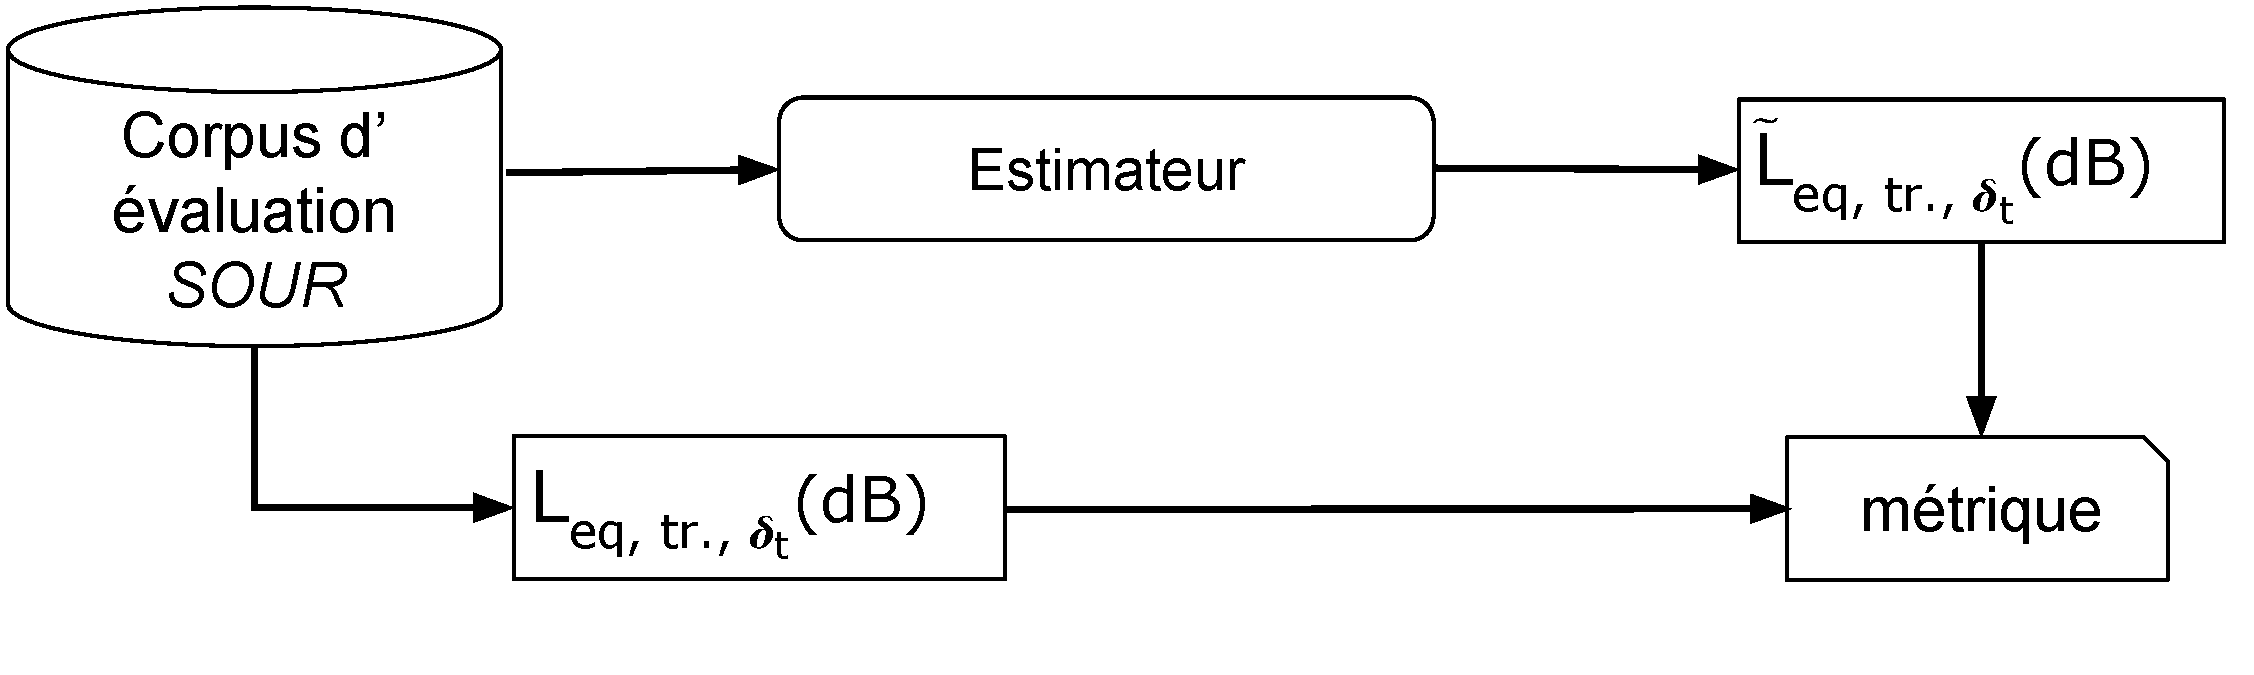
\includegraphics[width=0.9\linewidth]{./figures/NMF/Bloc_diagram_estimateur_SOUR.pdf}
\caption{Diagramme en blocs des étapes dans l'estimation du niveau sonore du trafic pour le corpus d'évaluation \textit{SOUR}.}
\label{fig:diagram_SOUR}
\end{figure}


De prime abord, les étapes mises en place dans cette partie sont similaires à celles du chapitre précédent et sont présentées dans la Figure \ref{fig:diagram_SOUR} : les scènes sonores du corpus d'évaluation \textit{SOUR} sont soumises à un estimateur qui détermine le niveau sonore du trafic estimé, $\tilde{L}_{eq,tr.}$ qui est comparé à sa valeur exacte, $L_{eq,tr.}$ par le calcul d'une métrique.
Le corpus d'évaluation \textit{SOUR}, présenté en détail dans la partie \ref{part:corpus_grafic}, est composé de 74 fichiers audio d'une durée totale de 2h50, divisé en 4 ambiances sonores : \textit{Parc} (8 scènes, abrégé \textit{Pa.}), \textit{Rue calme} (35 scènes, abrégé \textit{Ca.}), \textit{Rue bruyante} (23 scènes, abrégé \textit{Br.}), \textit{Rue très bruyante} (8 scènes, abrégé \textit{Tr. Br.}). Ce corpus a été réalisé à partir d'enregistrements sonores et de leurs annotations afin d'obtenir de scènes sonores simulées dont la structure temporelle est similaire à celle des scènes réelles. La qualité et le réalisme de ces scènes ont été validées grâce à un test perceptif. Ces scènes étant assimilables à des enregistrements sonores, elles permettent d'évaluer aux mieux les performances de la NMF face à de telles mixtures sonores. Comparé au corpus \textit{Ambiance}, ces scènes présentent une part du trafic plus importante et mélangent de multiples sources sonores (aboiement de chien, sifflement d'oiseaux, voix, bruit de rue, bruit de pas, sonnerie, portes \dots{}). Les sources sonores appartenant aux classes de sons interférantes \textit{climat} (vent, pluie, orage) et \textit{transport} (tramway, avion et train) ne sont pas présentes dans ce corpus.

Chaque scène du corpus est soumise à un estimateur qui détermine le niveau sonore du trafic routier. 
Le premier estimateur \textit{baseline} reste le même que dans le chapitre \ref{chap:ambiance} : un filtre passe-bas (abrégé filtre PB) de fréquence de coupure $f_c$ avec $f_c \in \lbrace 100,~500,~1k,~2k,~5k,~10k,~20k \rbrace$ Hz. Son application reste similaire : le spectrogramme du signal audio est coupé à la fréquence $f_c$ et toute l'énergie située dans la bande passante est assimilée au trafic routier (voir Figure \ref{fig:baseline}).
Le second estimateur est basé sur plusieurs formes de NMF : NMF supervisée (NMF SUP), semi-supervisée (NMF SEM) ainsi que la NMF seuillée initialisée (NMF IS). Le choix de la $\beta$-divergence reste circonscrit à $\beta \in \lbrace 0,~1,~2 \rbrace$.
L'apprentissage du dictionnaire suit les même étapes que dans le chapitre précédent : chaque spectrogramme, issu des 53 fichiers audio constituant le corpus d'apprentissage, est découpé en trames temporelles de durée $w_t \in \lbrace 0,5,~1,~2 \rbrace$ secondes. Les valeurs \textit{rms} sont ensuite calculées selon la fréquence. L'algorithme de clustering $K$-means est ensuite appliqué afin de fixer le nombre d'éléments dans $\mathbf{W}$ à $K \in \lbrace 25,~50,~100,~200,~ 300 \rbrace$. Le cas \textit{all}, où la valeur \textit{rms} est calculée sur l'intégralité du corpus, est aussi conservé avec la réduction des matrices restreinte à $K_{w_t = all} = \lbrace 25,~50 \rbrace$. Les dictionnaires, constitués d'éléments \textit{trafic}, composent les dictionnaires $\mathbf{W}$ de la NMF SUP, les dictionnaires $\mathbf{W_s}$ de la NMF SEM et les dictionnaires $\mathbf{W_0}$ de la NMF IS qui sont ensuite mis à jour.
Pour la NMF SEM, le nombre d'éléments dans le dictionnaire $\mathbf{W_r}$ est maintenu à $J = 2$.
Dans le cas de la NMF IS, l'influence de l'opérateur sigmoïde dans le calcul de la distance $D_{\theta}(\mathbf{W_0}\Vert \mathbf{W'})$ et l'utilisation du seuil \textit{firm} s'étant relevées très faibles, l'étude se réduit au seul cas de la représentation linéaire de la distante $D_{\theta}$ avec un seuillage dur de seuil $t_h$.
Comme les scènes sonores sont plus longues (de 1 à 3 minutes), le nombre d'itération est étendu à 200. 
Le résumé de ces facteurs expérimentaux et de leurs modalités respectives se trouve dans le Tableau \ref{tab:experimental_factorsNMF}. Dans le cas de l'estimateur \textit{baseline}, 28 associations de modalités sont réalisées (4 environnements sonores $\times$ 7 $f_c$). Pour l'estimateur NMF, c'est en tout 13 776 combinaisons qui sont possibles (4 environnements sonores $\times$ 3 $\beta$ $\times$ (3 $w_t$ $\times$ 4 $K$ + 1 $w_t$ $\times$ 2 $K_{w_t = all}$) $\times$ (2 méthode+ 41 $t_h$)).

\begin{table*}[t]
\centering
\caption{Facteurs expérimentaux et leurs modalités utilisés pour le corpus \textit{SOUR}.}
\resizebox{\textwidth}{!}{%
\begin{tabularx}{17.5cm}{L{3cm}@{}C{12cm}@{}C{2cm}@{}}
	\hline
    \textbf{\begin{tabular}[c]{@{}l@{}}Facteur \\ expérimentaux \end{tabular}} & \textbf{Modalités} & \begin{tabular}[c]{@{}C{2cm}@{}}\textbf{Nombre de}\\ \textbf{modalités}\end{tabular}\\ \toprule
\end{tabularx}}

\resizebox{\textwidth}{!}{%
\begin{tabularx}{17.5cm}{L{3cm}@{}C{3cm}@{}@{}C{3cm}@{}@{}C{3cm}@{}@{}C{3cm}@{}C{2cm}@{}}
    \textbf{Environnement sonore} & \begin{tabular}[c]{@{}c@{}}parc\\ 'Pa'\end{tabular} & \begin{tabular}[c]{@{}c@{}}rue calme \\ 'Ca'\end{tabular} & \begin{tabular}[c]{@{}c@{}}rue bruyante\\ 'Br' \end{tabular}& \begin{tabular}[c]{@{}c@{}}rue très bruyante\\ 'Tr Br'\end{tabular} & 4\\
\end{tabularx}}

\resizebox{\textwidth}{!}{%
\begin{tabularx}{17.5cm}{L{3cm}@{}C{3cm}@{}@{}C{3cm}@{}@{}C{3cm}@{}@{}C{3cm}@{}C{2cm}@{}}
	\rowcolor[HTML]{C0C0C0}
  \textbf{Méthode} & filtre passe bas & NMF SUP & NMF SEM & NMF IS & 4\\
\end{tabularx}}

\resizebox{\textwidth}{!}{%
\begin{tabularx}{17.5cm}{L{3cm}@{}@{}C{1.714cm}@{}@{}C{1.714cm}@{}@{}C{1.714cm}@{}@{}C{1.714cm}@{}@{}C{1.714cm}@{}@{}C{1.714cm}@{}@{}C{1.714cm}@{}C{2cm}@{}}
   $\mathbf{f_c}$ (kHz) & 1 & 0.5 & 1 & 2 &  5 & 10 & 20 & 7\\
\end{tabularx}}

\resizebox{\textwidth}{!}{%
\begin{tabularx}{17.5cm}{L{3cm}@{}C{3cm}@{}@{}C{3cm}@{}@{}C{3cm}@{}@{}C{3cm}@{}C{2cm}@{}}
\rowcolor[HTML]{C0C0C0}
    $\mathbf{w_t}$ (s)& 0.5 & 1 & 2 & \textit{all} & 4\\
\end{tabularx}}

\resizebox{\textwidth}{!}{%
\begin{tabularx}{17.5cm}{L{3cm}@{}C{2.4cm}@{}@{}C{2.4cm}@{}@{}C{2.4cm}@{}@{}C{2.4cm}@{}@{}C{2.4cm}@{}C{2cm}@{}}
    $\mathbf{K}$ & 25 & 50 & 100 & 200 & 300 & 5\\
\end{tabularx}}

\resizebox{\textwidth}{!}{%
\begin{tabularx}{17.5cm}{L{3cm}@{}C{4cm}@{}@{}C{4cm}@{}@{}C{4cm}@{}C{2cm}@{}}
\rowcolor[HTML]{C0C0C0}
   $\mathbf{\beta}$ & 0 & 1 & 2 & 3\\
\end{tabularx}}

\resizebox{\textwidth}{!}{%
\begin{tabularx}{17.5cm}{L{3cm}@{}C{12cm}@{}C{2cm}@{}}
   seuillage dur $\mathbf{t_h}$ & de 0.20 à 0.60 avec un pas de 0.01 & 41\\
   \bottomrule
\end{tabularx}}

\label{tab:experimental_factorsNMF}
\end{table*}

 
En sortie de l'estimateur est calculé un niveau sonore global du trafic, $\tilde{L}_{eq,tr.,\delta_t}$. Dans le précédent corpus, comme chaque scène possédait une durée similaire de 30 secondes, les niveaux sonores équivalent étaient calculés pour une durée d'intégration $\delta_t$ de 30 secondes aussi. Ici, la durée des scènes dans le corpus \textit{SOUR} est variable, il serait donc moins rigoureux de comparer entre eux les niveaux sonores équivalents des différentes scènes intégrés sur leurs durées totales si celles-ci sont différentes. La scène la plus courte dure 55 secondes (scène n$^{\circ}$ 14 de l'ambiance \textit{rue très bruyante}) et la plus longue dure 270 secondes (scène n$^{\circ}$ 4 de l'ambiance \textit{rue très bruyante} également). Pour harmoniser le calcul de la métrique, c'est un niveau sonore équivalent qui est calculé avec une durée d'intégration $\delta_t$ de 60 secondes : 

\begin{equation}
L_{eq,tr.,60s} = 10 \times \log_{10}\left(\frac{1}{60}\int_{t_{init}}^{t_{init}+60} 10^{L_{p,tr.}(t)/10} dt\right)
\end{equation}

avec $L_{p,tr.}(t)$ l'expression du niveau sonore.
Pour chaque ambiance sonore, les signaux \textit{trafic} obtenus en sortie de l'estimateur sont concaténés les uns aux autres. Puis le niveau sonore équivalent est successivement calculé toutes les 60 secondes. Il est alors possible de déterminer un niveau sonore $L_{eq,tr.,60s}$ dont une partie est calculée sur une scène et l'autre partie sur la scène suivante. On résume, en Figure \ref{fig:exempe_mae60}, un exemple du procédé. 

\begin{figure}[h!]
\centering
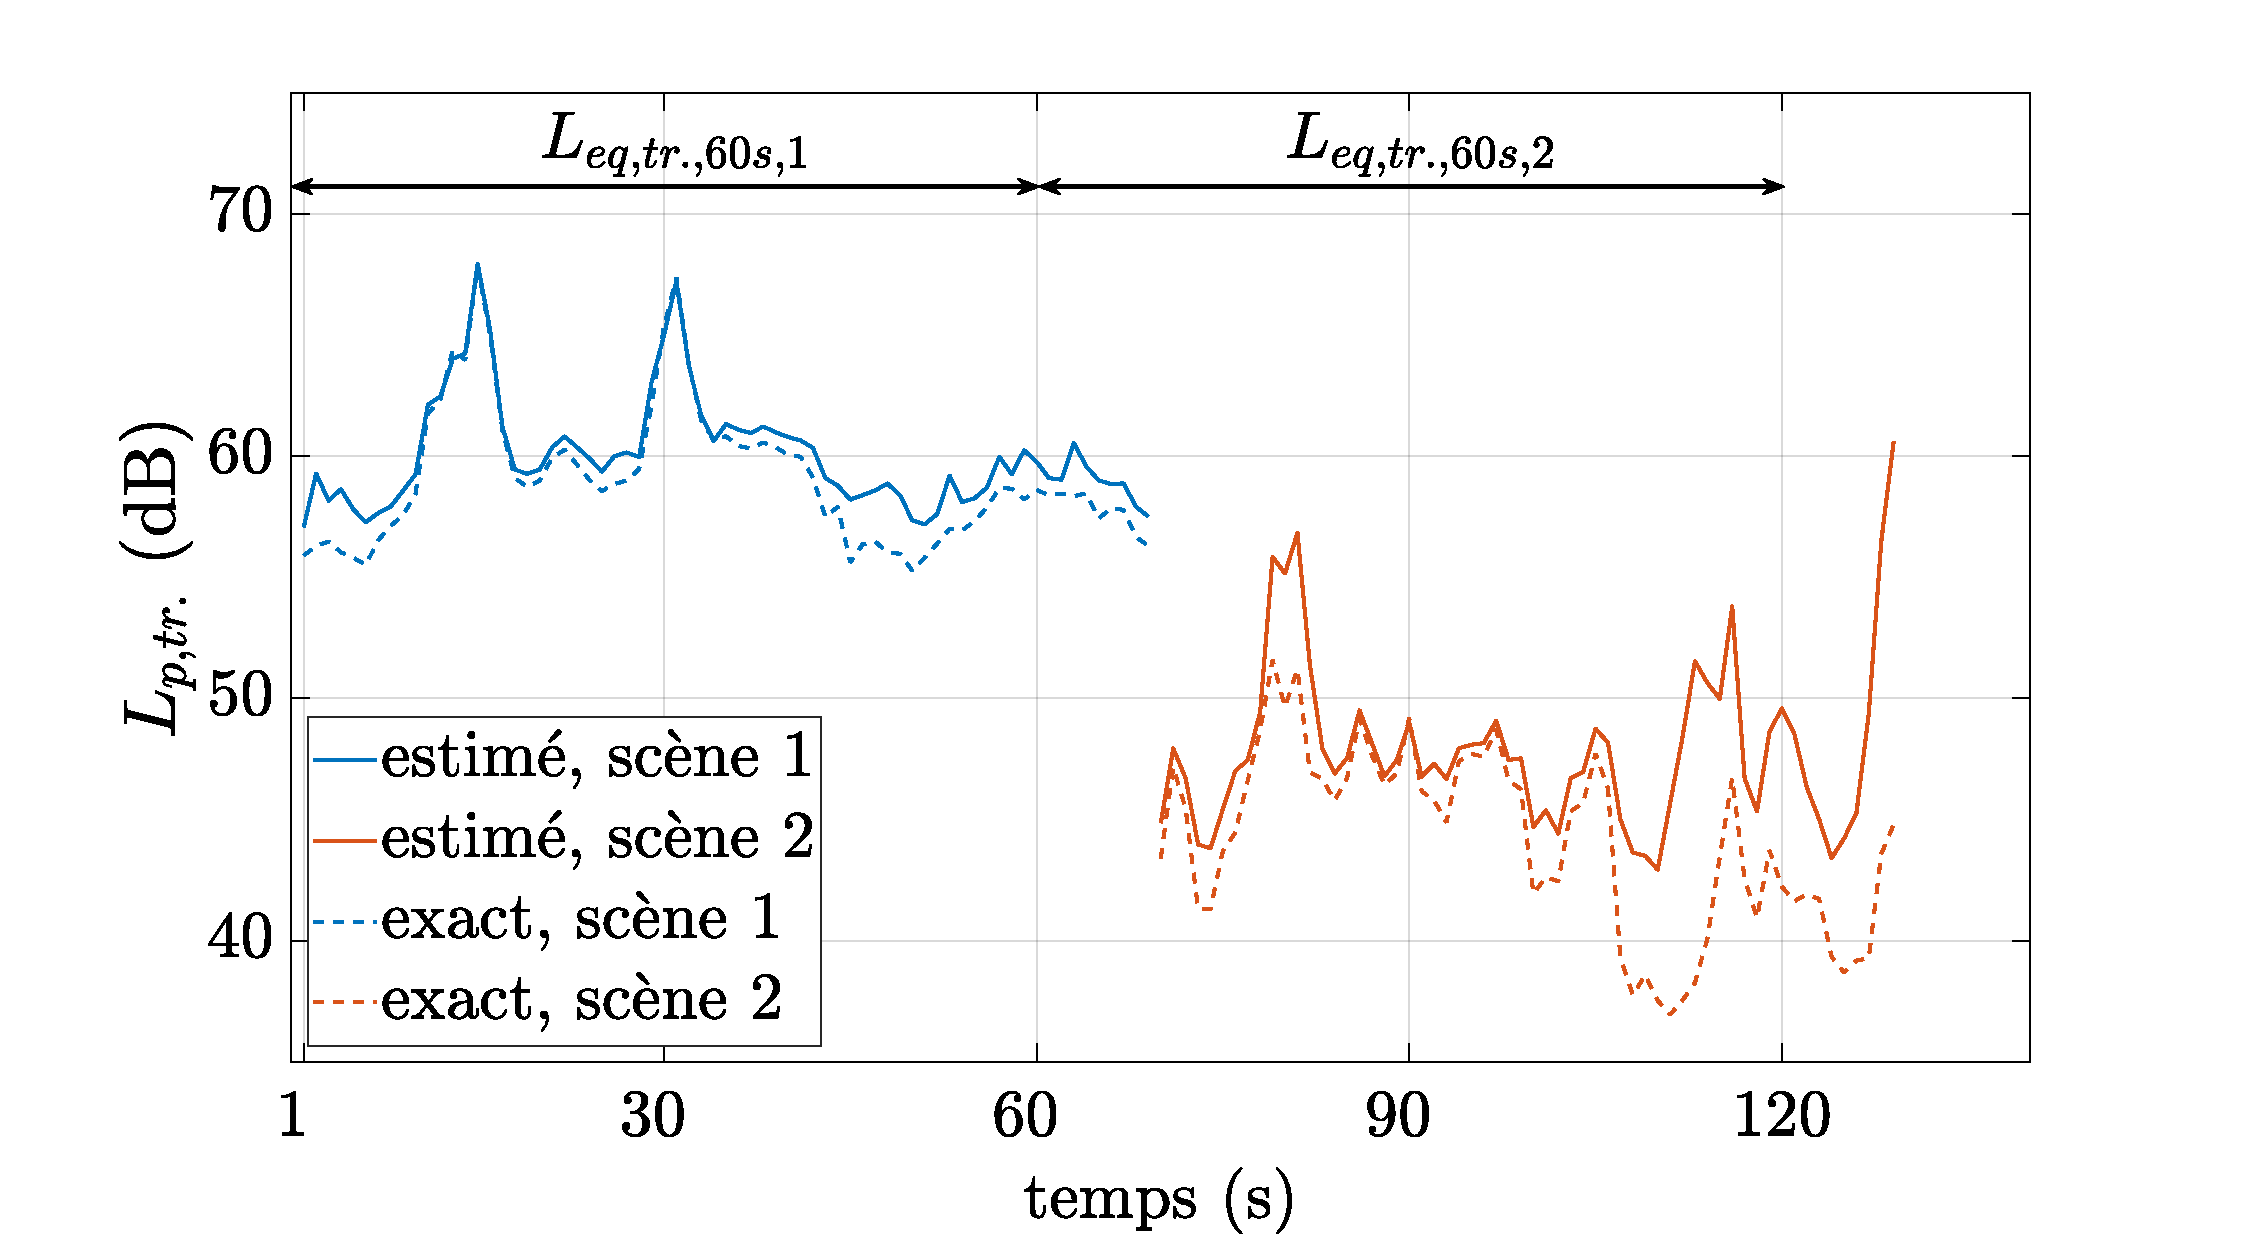
\includegraphics[width=.9\linewidth]{./figures/resultats/Lp_mae.pdf}
\caption{Estimation des niveaux sonores équivalents pour une durée d'intégration de 60 secondes sur deux scènes. Le deuxième niveau sonore inclut 9 secondes de la scène 1 et 51 secondes de la scène 2.}
\label{fig:exempe_mae60}
\end{figure}

Le nombre d'erreurs calculées par ambiance est donc différent du nombre de scènes qui la compose. Le Tableau \ref{tab:resume_sour} récapitule le nombre de scènes par ambiance ainsi que leur durée cumulée et le nombre de niveaux sonores équivalent à la minute calculé en conséquence ($N_{60}$).

\begin{table}[h!]
\caption{Corpus d'évaluation \textit{SOUR} avec le nombre d'erreur $MAE_{60}$ calculé.}
\label{tab:resume_sour}
\centering
\begin{tabular}{L{3cm}C{2cm}C{2cm}C{2cm}C{2cm}C{2cm}}
\toprule
Ambiance sonore & Parc & Calme & Bruyant & Très Bruyant & Total\\ \midrule
$N$ & 8 & 35 & 23 & 8 & 74 \\
durées (s) & 960 & 4636 & 3366 & 1285 & 247 \\
$N_{60}$ & 16 & 77 & 56 & 21 & 160 \\ \bottomrule
\end{tabular}
\end{table}

L'erreur $MAE_{60}$ est calculé pour chaque association de modalité pour chaque ambiance sonore : 

\begin{equation}
MAE_{60} = \frac{\sum_{i = 1}^{N_{60}}\vert L_{eq,tr.,60s, i} - \tilde{L}_{eq,tr.,60s, i}\vert}{N_{60}}
\end{equation}

Cette erreur est ensuite moyennée sur l'intégralité des ambiances sonores pour déterminer la combinaison de modalités optimale qui permet l'erreur la plus faible sur l'ensemble du corpus :
  
\begin{equation}
MAE_{g} = \frac{\sum_{j = 1}^4 MAE_{60,j}}{4}.
\end{equation}

Le choix a été fait de ne pas pondérer l'erreur $MAE_{g}$ selon le nombre $N_{60}$ par ambiance. Par leur durée plus importante, une moyenne pondérée serait plus influencée par les ambiances \textit{rue calme} et \textit{rue bruyante}. Afin de déterminer la combinaison la plus efficace sur l'ensemble des ambiances, le même poids est donc donné à chaque ambiance sonore.



\section{Erreurs $MAE_g$ obtenues par l'estimateur \textit{baseline}}
Dans un premier temps, les erreurs réalisées par l'estimateur \textit{baseline} sont observées sur l'ensemble du corpus et selon chaque ambiance (Tableau \ref{tab:grafic_baseline}).

\begin{table}[h]
\caption{Erreurs moyennes $MAE_{g}$ et $MAE_{60}$ pour l'estimateur \textit{baseline} pour le corpus d'évaluation \textit{SOUR}.}
\label{tab:grafic_baseline}
\centering
\resizebox{\textwidth}{!}{%
\begin{tabular}{L{1.3cm}C{2.85cm}@{}C{2.85cm}@{}C{2.85cm}@{}C{2.85cm}@{}C{2.85cm}}
\toprule
$f_c$ (Hz) & $MAE_{g}$ & $MAE_{60,Pa}$ & $MAE_{60,Ca}$ & $MAE_{60,Br}$  & $MAE_{60,TrBr}$ \\
\midrule
100 & 2,89 ($\pm$ 0,56) & \textbf{2,48 ($\pm$ 1,85)} & 3,71 ($\pm$ 2,63) & 2,66 ($\pm$ 1,20) & 2,70 ($\pm$ 0,71 )\\
 \rowcolor[HTML]{C0C0C0}
500 & \textbf{\textcolor{red}{1,99 ($\pm$ 1,37)}} & 3,87 ($\pm$ 5,08) & \textbf{2,14 ($\pm$ 2,25)} & 1,03 ($\pm$ 0,53) & 0,93 ($\pm$ 0,38) \\
1k & 2,44 ($\pm$ 2,57) & 6,07 ($\pm$ 5,26) & 2,46 ($\pm$ 2,81) & \textbf{0,64 ($\pm$ 0,64)} & 0,59 ($\pm$ 0,37) \\
 \rowcolor[HTML]{C0C0C0}
2k & 2,99 ($\pm$ 3,28) & 7,60 ($\pm$ 5,28) & 3,01 ($\pm$ 2,93) & 0,95 ($\pm$ 0,97) & \textbf{0,39 ($\pm$ 0,54)} \\
5k & 3,48 ($\pm$ 3,84) & 8,89 ($\pm$ 5,22) & 3,48 ($\pm$ 3,12) & 1,13 ($\pm$ 1,10) & 0,42 ($\pm$ 0,64) \\
 \rowcolor[HTML]{C0C0C0}
10k & 3,59 ($\pm$ 3,93) & 9,11 ($\pm$ 5,29)& 3,64 ($\pm$ 3,19) & 1,17 ($\pm$ 1,14) & 0,43 ($\pm$ 0,66) \\
20k & 3,62 ($\pm$ 3,93) & 9,14 ($\pm$ 5,31) & 3,68 ($\pm$ 3,20) & 1,21 ($\pm$ 1,14) & 0,44 ($\pm$ 0,67) \\
\bottomrule         
\end{tabular}}
\end{table}

De même que dans le chapitre précédent, c'est le filtre PB à la fréquence de coupure $f_c$ = 500 Hz qui génère l'erreur $MAE_g$ la plus faible ($MAE_g$ = 2,03 ($\pm$ 1,43)) en réalisant un compromis entre l'énergie rejetée dans les ambiances \textit{Parc} et \textit{Rue calme} et l'énergie conservée dans les deux autres ambiances. En détaillant les erreurs $MAE_{60}$ selon chaque ambiance, on retrouve un comportement similaire à celui observé pour le corpus \textit{ambiance} : plus la contribution de la source \textit{trafic} est présente, plus la fréquence de coupure, nécessite d'être augmentée. 
On remarque enfin que l'erreur $MAE_g$ à 20 kHz excède 3 dB, valeur qui correspond à la marge d'incertitude acceptée des niveaux de bruits. Cette erreur démontre donc bien que, sans le traitement de données, la construction de cartes de bruit trafic sur des mesures serait imparfaite.

\section{Erreurs $MAE_g$ obtenues par l'estimateur NMF}
\label{chap:grafic_nmf}

Les erreurs générées par l'estimateur NMF selon les multiples associations des modalités des facteurs expérimentaux sont maintenant détaillées. Devant le nombre important de résultats, on ne détaille dans le Tableau \ref{tab:erreur_mae60} que les résultats les plus performants selon chaque méthode (NMF SUP, SEM et IS) et les 3  valeurs de $\beta$. 

\begin{table}[h]
\centering
\caption{Erreurs $MAE_{60}$ pour les combinaisons optimales de modalités des estimateurs pour le corpus d'évaluation \textit{SOUR}.}
\label{tab:erreur_mae60}
\begin{tabular}{L{2cm}C{1.5cm}C{1.2cm}C{1.2cm}C{1.2cm}C{1.2cm}C{2.5cm}C{2.5cm}}
\toprule
méthode & $f_c$ (kHz) & $\beta$ & $w_t$ & K & $t_h$ & $MAE_{60}$ \\ \toprule
\multirow{2}{*}{filtre PB} & 20 & - & - & - & - &  3,62 ($\pm$ 3,93) \\
 & 0,5 & - & - & - & - & 1,99 ($\pm$ 1,37) \\ \midrule
\multirow{3}{*}{NMF SUP} & - & 0 & 0,5 & 200 & - & 3,13 ($\pm$ 3,33) \\
 & - & 1 & 0,5 & 200 & - & 2,67 ($\pm$ 3,02) \\
 & - & 2 & 0,5 & 25 & - & 2,13 ($\pm$ 2,22) \\ \midrule
\multirow{3}{*}{NMF SEM} & - & 0 & 0,5 & 300 & - & 2,02 ($\pm$ 0,68) \\
 & - & 1 & 0,5 & 300 & - & 1,93 ($\pm$ 0,42) \\
 & - & 2 & 1 & 300 & - & 2,24 ($\pm$ 0,89) \\ \midrule
\multirow{3}{*}{NMF IS} & - & 0 & 1 & 25 & 0,34 & 1,50 ($\pm$ 1,16) \\
 & - & 1 & 1 & 200 & 0,35 &  1,31 ($\pm$ 1,02) \\
 & - & \textbf{2} & \textbf{1} & \textbf{300} & \textbf{0,35} & \textbf{\textcolor{red}{1,16 ($\pm$ 0,86)}} \\
 \bottomrule
\end{tabular}
\end{table}

La composition du corpus \textit{SOUR} étant différente de celle du corpus \textit{Ambiance}, les combinaisons optimales diffèrent de celles obtenues dans le chapitre précédent dans certains cas.
La NMF SUP reste la méthode la moins performante avec des erreurs supérieures à celles de l'estimateur \textit{baseline} à $f_c$ = 500 Hz avec des écart-types plus importants notamment pour l'estimateur basé sur la divergence d'Itakura-Saïto ($\beta$ = 0). Contrairement au corpus \textit{Ambiance} où chaque approche privilégie un dictionnaire comprenant un faible nombre d'éléments, ici, la NMF SUP avec $\beta \in \lbrace 0,~1 \rbrace$ choisit un nombre plus élevé d'éléments ($K$ = 200). Seul la NMF basée sur la distance EUC conserve un faible nombre d'éléments.
%Dans le précédent corpus en faisant l'erreur moyenne seulement pour les $TIR$ positifs on obtient, parmi les meilleurs combinaisons des dictionnaires composé d'un plus grand nombre d'éléments. Le corpus SOUR étant composé de plus de scènes dont le trafic est plus présent, ces méthodes peuvent donc privilégié un dictionnaire composé de plus d'éléments \textit{trafic}.

Les versions optimales de la NMF SEM sont basées sur le même dictionnaire et privilégient un grand nombre d'éléments dans le dictionnaire ($K$ = 300). Leur erreurs ne diffèrent donc que par le choix de $\beta$. Ces modalités restent ici cohérentes par rapport au corpus précédent où c'était également un dictionnaire unique composé d'un grand nombre d'éléments, qui offrait les erreurs les plus faibles.  Toutefois, si la NMF SEM permet des erreurs plus faibles que la NMF SUP, elle n'améliore pour autant  les performances de l'estimateur \textit{baseline} que pour $\beta$ = 1.  

La NMF IS se révèle être l'approche la plus performante avec systématiquement, pour les trois valeurs de $\beta$, des erreurs $MAE_g$ inférieures à 1,5. La méthode la plus performante est celle basée sur la distance EUC avec $K$ = 300, $w_t$ = 1 s et un seuil $t_h$ = 0,35 et génère une erreur $MAE_g$ de 1,19 ($\pm$ 0,91). On constate que pour $\beta = 0$, à l'inverse du corpus \textit{Ambiance}, le nombre d'éléments est ici réduit à 25. 
Les valeurs seuils sont également plus faibles pour ce corpus \textit{SOUR} puisque la part du trafic est ici plus importante que dans le corpus \textit{Ambiance}. De plus, les classes de sons dans le corpus \textit{SOUR} appartiennent majoritairement aux classes interférantes \textit{alerte}, \textit{animaux} et \textit{humains}, des classes de sons dont les spectres sont moins similaires à ceux du trafic. En conséquence, la distance $D_{\theta}$ entre les éléments \textit{trafic} et ceux modélisant ces sources est plus faible. 
La NMF IS avec $\beta$ = 2, $K$ = 300, $w_t$ = 1 s et $t_h$ = 0,35 est donc l'approche qui génère la plus faible erreur de reconstruction sur l'ensemble du corpus d'évaluation \textit{SOUR}. Les combinaisons optimale de la NMF SUP ($\beta$ = 2, $K$ = 25 et $w_t$ = 0,5 s) et de la NMF SEM ($\beta$ = 1, $K$ = 300, $w_t$ = 2) génèrent des erreurs plus importantes et ne sont donc pas des estimateurs adéquats pour cette tâche.

\begin{figure}[h!]
\centering
\subfigure[Fonction de coût moyen pour le corpus élémentaire \textit{SOUR} selon les 3 NMF optimales retenues.]{%
\label{fig:cost_grafic}%
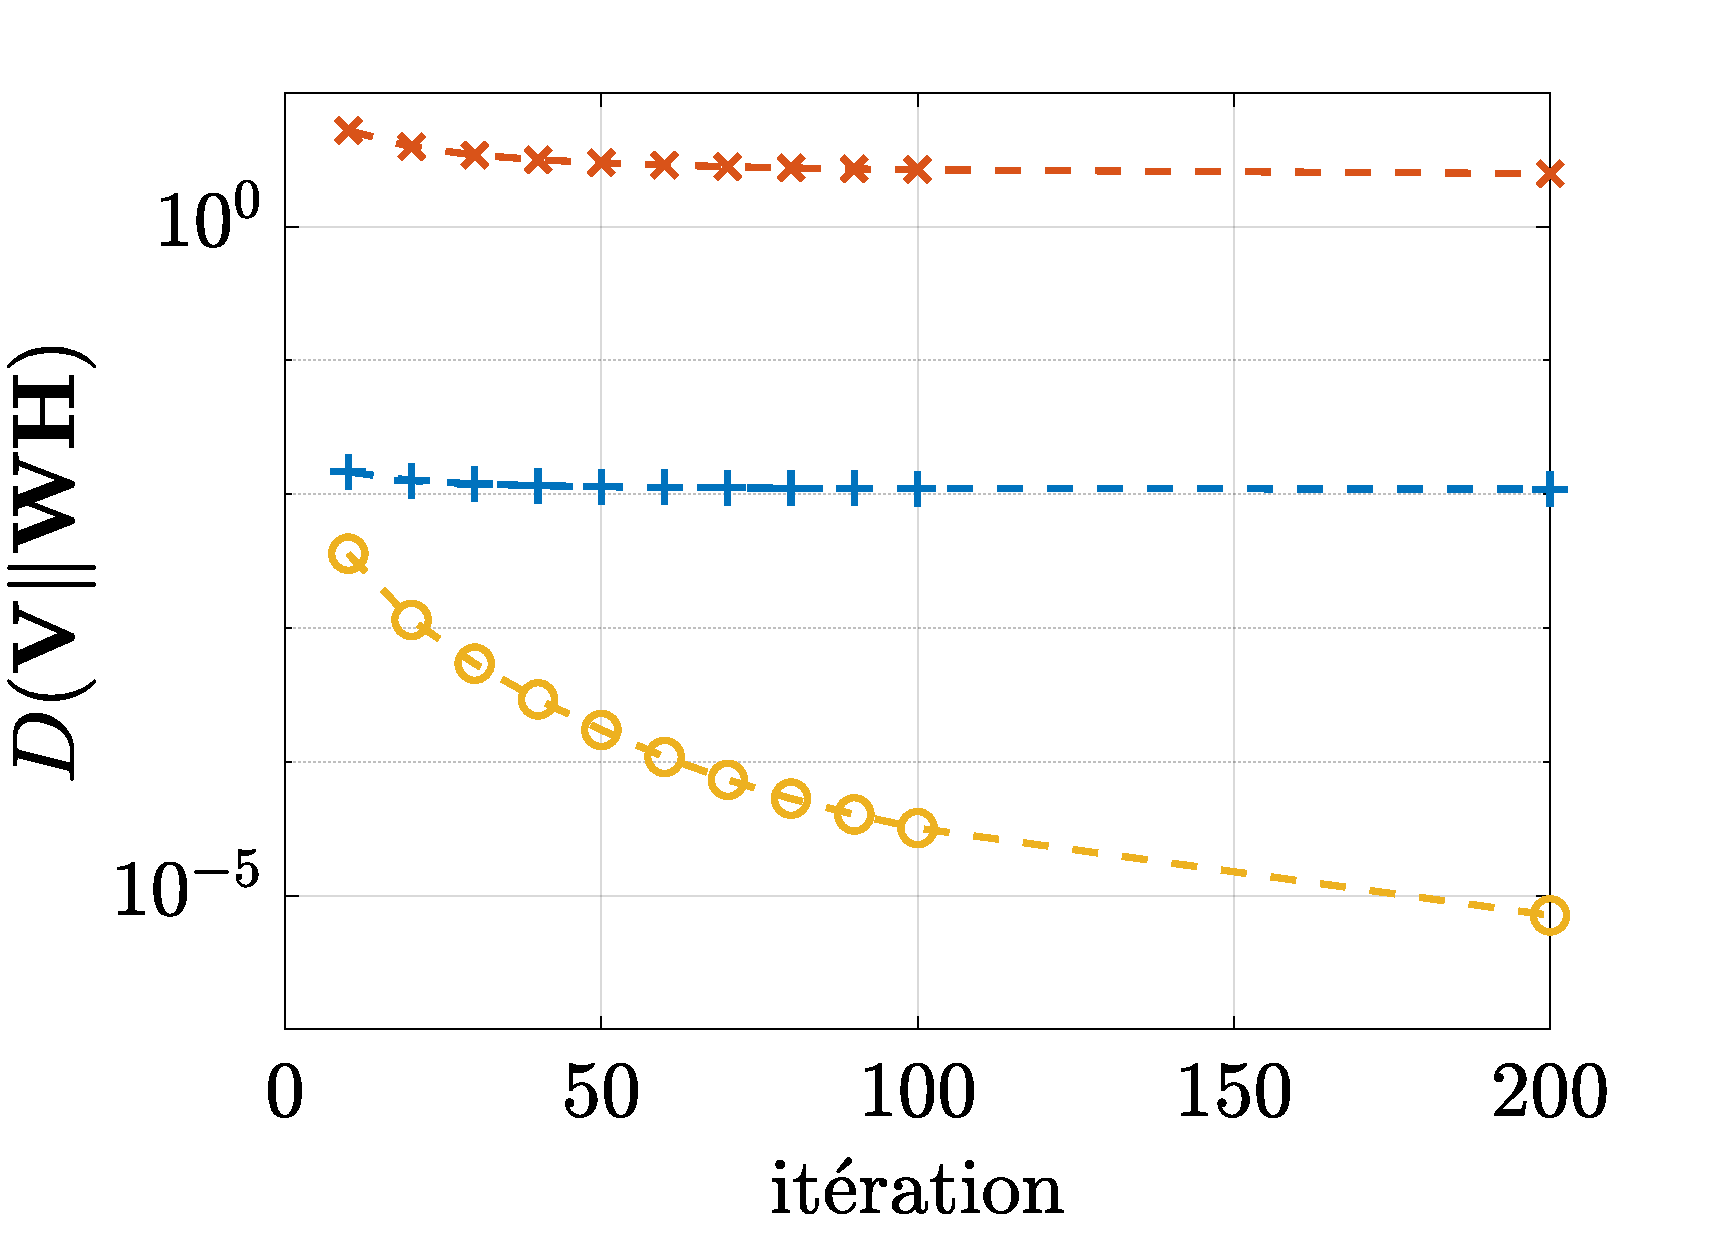
\includegraphics[width=.45\linewidth]{./figures/resultats/grafic_cost.pdf}}%
\qquad
\subfigure[Évolution de l'erreur $MAE_g$ pour les 3 NMF optimales retenues.]{%
\label{fig:mae_grafic}%
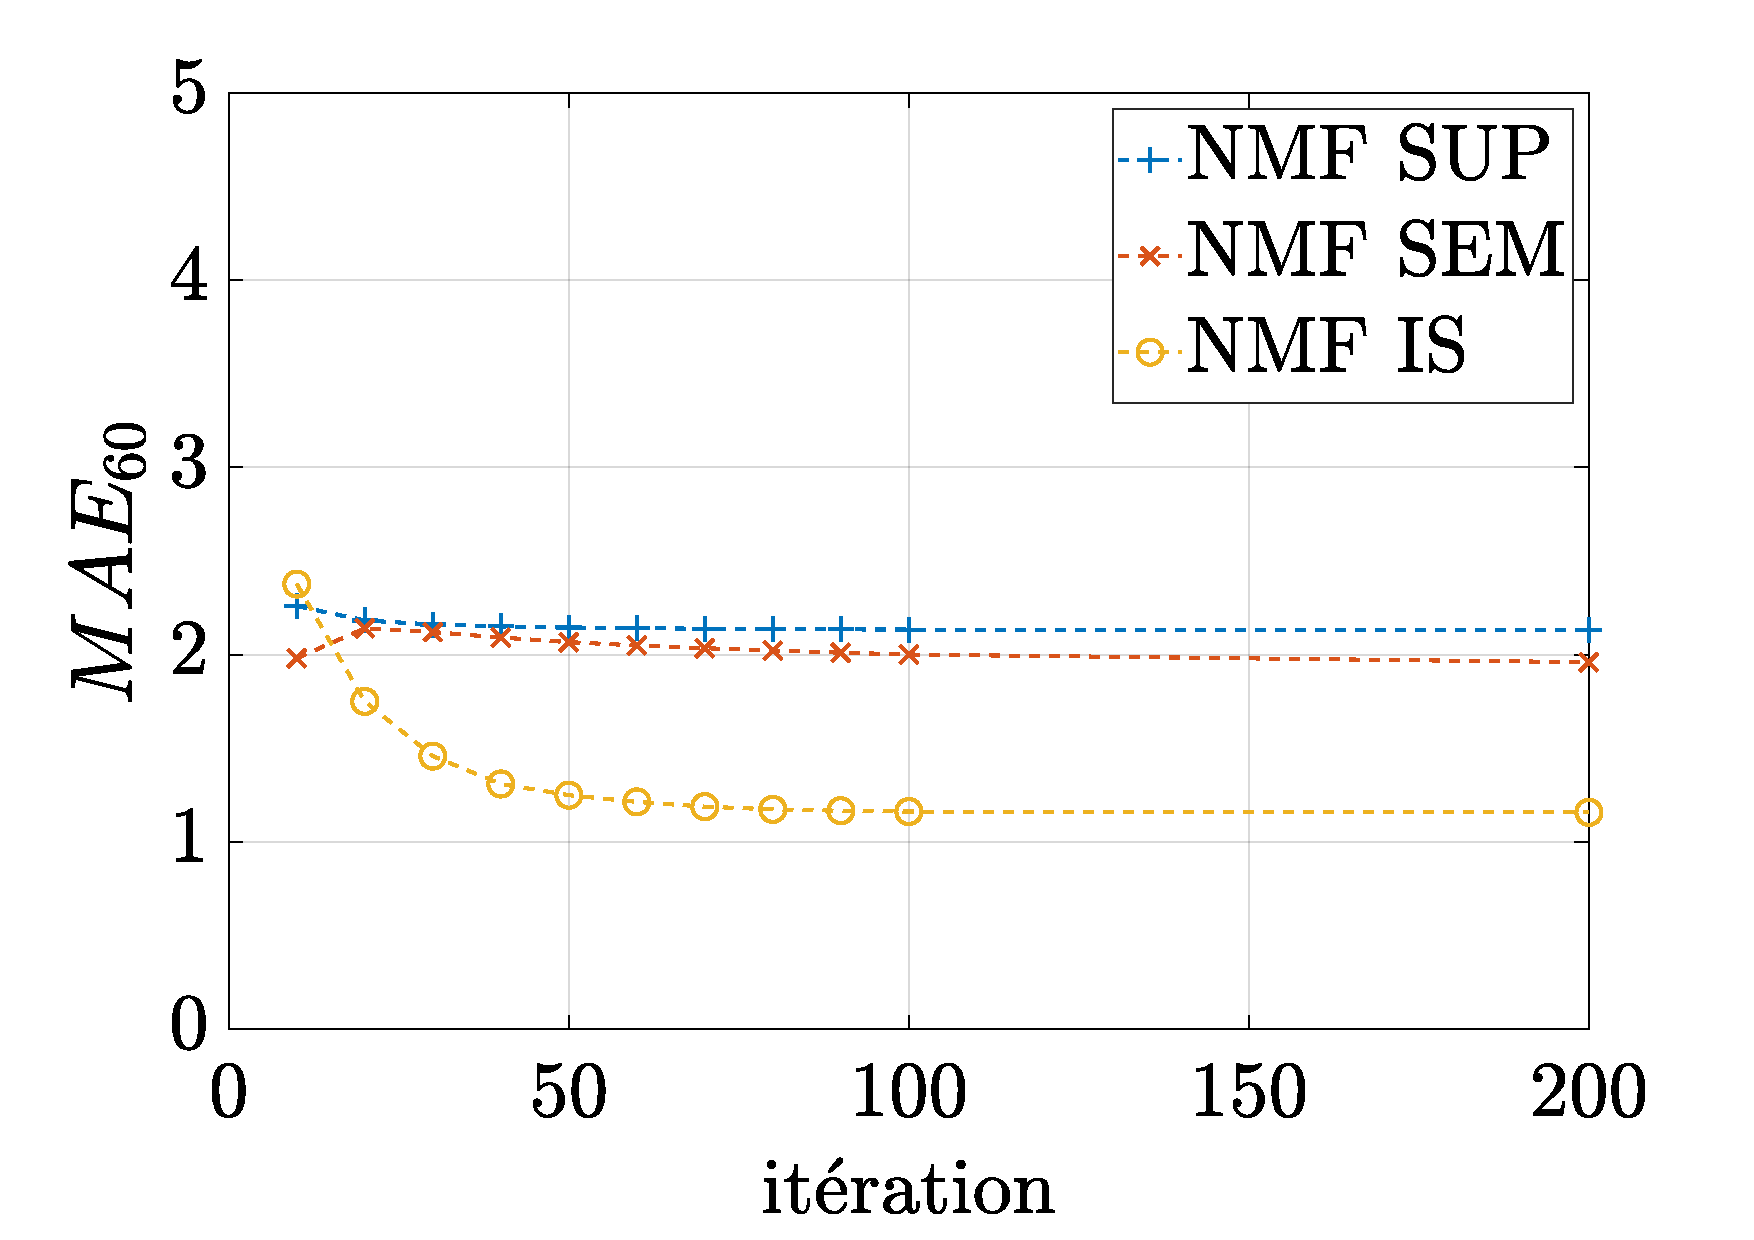
\includegraphics[width=.45\linewidth]{./figures/resultats/mae_grafic.pdf}}%
\caption{Influence de la forme du dictionnaire pour les 3 NMF retenues.}
\label{fig:evolution_mae}
\end{figure}

Les erreurs de reconstruction $D(\mathbf{V} \Vert \mathbf{WH})$ ainsi que l'évolution de l'erreur $MAE_g$ en fonction des itérations sont présentées en Figure \ref{fig:evolution_mae}. La fonction de coût est naturellement meilleure pour la NMF IS puisque les matrices $\mathbf{W}$ et $\mathbf{H}$ sont mises à jour. Si la convergence n'est pas atteinte au bout de 200 itération, l'erreur $MAE_{60}$ est pour autant constante. Entre la NMF SUP et SEM, l'erreur de reconstruction est rapidement stable après 100 itérations. 
Grâce à la partie mobile $\mathbf{W_r}$ dans le dictionnaire de la NMF SEM, l'approche permet de mieux s'adapter aux différentes scènes et donc de diminuer la valeur de la fonction de coût. À l'inverse, la NFM SUP est contrainte de réaliser la reconstruction du signal avec les éléments fixes de son dictionnaire. Ayant moins de souplesse, l'erreur de reconstruction est plus élevée. Ce comportement se retrouve également dans l'évolution de l'erreur $MAE_{60}$ : ayant une meilleure reconstruction globale du signal, la NMF IS obtient aussi des erreurs plus faibles. 

\section{Erreurs par ambiance sonore}

L'erreur par ambiance sonore est ensuite détaillée selon les combinaisons optimales de chaque NMF : 

\begin{itemize}
\item NMF SUP, $\beta$ = 2, $w_t$ = 0,5 s, $K$ = 25,
\item NMF SEM, $\beta$ = 1, $w_t$ = 0,5, $K$ = 300,
\item NMF IS, $\beta$ = 2, $w_t$ = 1, $K$ = 300.
\end{itemize}

 Le temps de calcul mis par l'estimateur pour extraire la composante \textit{trafic} d'un spectrogramme $\mathbf{V}$ d'une durée de 1 minute est ajouté. Dans le cas de la NMF, c'est le temps mis par la méthode pour réaliser les 200 itérations. Le Tableau \ref{tab:erreur_mae60_amb} résume les erreurs $MAE_{60}$ pour chaque ambiance. Les erreurs générées par l'estimateur \textit{baseline} à $f_c$ = 500 Hz et $f_c$ = 20 kHz sont également ajoutées.

\begin{table}[h]
\centering
\caption{Erreurs $MAE_{60}$ selon les estimateurs NMF pour chaque méthode dans sa combinaison optimale de modalités avec les estimateurs \textit{baseline} à 500 Hz et 20 kHz. En gras-rouge, les erreurs les plus faibles, en gras-noir, les erreurs de la NMF inférieures à l'estimateur \textit{baseline} $f_c$ = 500 Hz.}
\label{tab:erreur_mae60_amb}
\resizebox{\textwidth}{!}{%
\begin{tabular}{L{4cm}C{2.5cm}C{2.5cm}C{2.5cm}C{2.5cm}C{2.5cm}}
\toprule
méthode & Parc & Rue Calme & Rue Bruyante & Rue très bruyante & temps de calcul/min (s)\\ \midrule
filtre PB, $f_c$ = 20 kHz & 9,14 ($\pm$ 5,31) & 3,68 ($\pm$ 3,20) & 1,21 ($\pm$ 1,14) & 0,44 ($\pm$ 0,67) &  0,03 ($\pm$ 0,01) \\
filtre PB, $f_c$ = 500 Hz & 3,87 ($\pm$ 5,08) & 2,14 ($\pm$ 2,25) & 1,03 ($\pm$ 0,53) & 0,93 ($\pm$ 0,38) &  0,03 ($\pm$ 0,01) \\ \midrule
NMF SUP & 5,31 ($\pm$ 5,06)  & 2,02 ($\pm$ 2,22) & \textbf{0,62 ($\pm$ 0,56)} & \textbf{0,57 ($\pm$ 0,33)} & 0,09 ($\pm$ 0,03)\\
NMF SEM & \textbf{2,50 ($\pm$ 2,71)} & 2,36 ($\pm$ 2,42) & 1,62 ($\pm$ 0,87) & 1,42 ($\pm$ 0,60) & 1,77 ($\pm$ 0,13)\\
NMF IS & \textbf{\textcolor{red}{2,13 ($\pm$ 3,84)}} & \textbf{\textcolor{red}{1,62 ($\pm$ 1,85)}} & \textbf{\textcolor{red}{0,57 ($\pm$ 0,54)}} &  \textbf{\textcolor{red}{0,32 ($\pm$ 0,20)}} & 2,15 ($\pm$ 0,31)\\ \bottomrule
\end{tabular}}
\end{table}

Dans le chapitre précédent, la NMF IS était sur l'intégralité du corpus la méthode générant l'erreur moyenne la plus faible mais elle ne permettait pas d'obtenir les plus faibles erreurs selon chaque $TIR$. La NMF SEM optimale générait alors les erreurs les plus faibles dans les $TIR$ négatifs et la NMF SUP supplantait les autres méthodes pour les $TIR$ positifs. 
Sur le corpus \textit{SOUR}, la NMF IS se révèle être la méthode obtenant les plus faibles erreurs sur l'ensemble des ambiances sonores. Elle parvient notamment à être plus performante que le filtre à 20 kHz dans l'ambiance \textit{Rue très bruyante}. 

\begin{figure}[h]
\centering
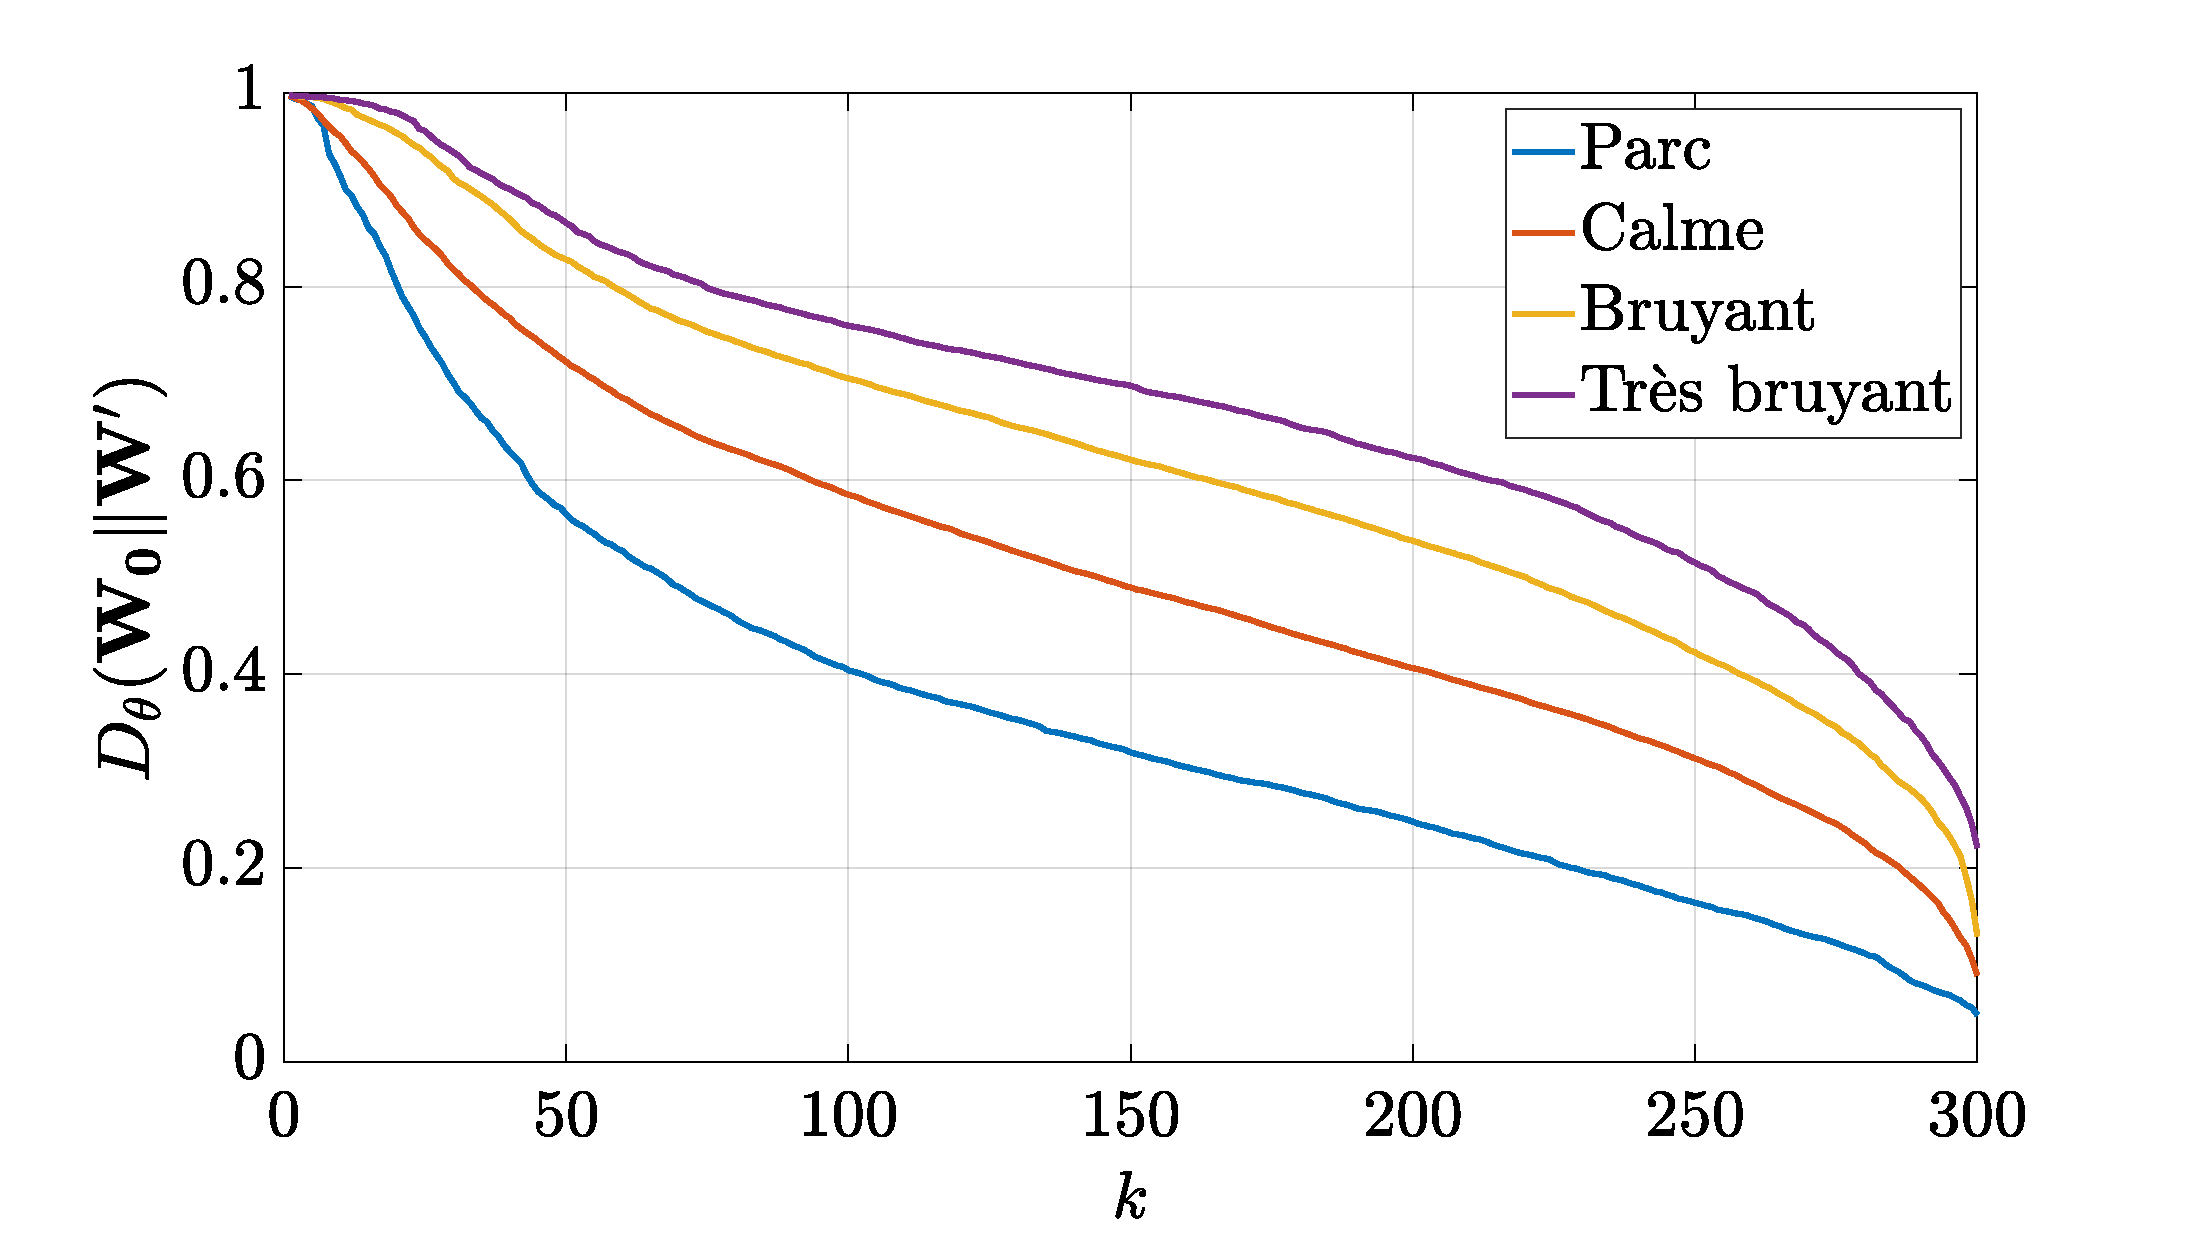
\includegraphics[width=.7\linewidth]{./figures/resultats/dist_grafic.pdf}
\caption{Distances $D_{\theta}(\mathbf{W_0}\Vert \mathbf{W'})$ moyennes par ambiance sonore triées par ordre décroissant  dans le cas de la NMF IS optimale ($\beta$ = 2, $K$ = 300, $w_t$ = 1).}
\label{fig:dist_grafic}
\end{figure}

Le comportement de la NMF IS peut s'illustrer au travers des évolutions de la distance $D_{\theta}$ moyenne pour chaque ambiance sonore (Figure \ref{fig:dist_grafic}).
En fixant un seuil sur l'ensemble des ambiances sonores, le nombre d'éléments inclut dans $\mathbf{W}_{trafic}$ est variable. 
Dans le cas de l'ambiance \textit{Très bruyant}, le nombre d'éléments moyen est de 286 soit quasiment l'intégralité du dictionnaire $\mathbf{W'}$. Ce nombre est justifié par le fait que le trafic est la source sonore dominante dans ces scènes : $\mathbf{W'}$ dévie donc moins de $\mathbf{W_0}$. En utilisant un seuil bas, on conserve suffisamment d'éléments dans $\mathbf{W}_{trafic}$ pour bien modéliser la source \textit{trafic}.
Dans le cas de l'ambiance \textit{Parc}, étant composée de peu d'éléments appartement à la classe de sons \textit{trafic}, la distance $D_{\theta}$ dévie beaucoup plus réduisant le nombre d'éléments de $\mathbf{W'}$ inclus dans $\mathbf{W}_{trafic}$ à 130.

Les deux autres NMF sont moins performantes.
Le comportement de la NMF SUP reste similaire à celui observé dans le chapitre précédent : elle échoue à améliorer les erreurs de l'estimateur \textit{baseline} dans les ambiances où le trafic est peu présent mais offre de meilleures performances lorsque le trafic devient la source sonore principale grâce à son dictionnaire composé de spectres de trafic.
La NMF SEM est finalement, sur ce corpus et sur les 3 NMF comparées, celle qui offre les résultats les moins bons. Si l'erreur obtenue dans l'ambiance \textit{Parc} reste limitée, avec l'augmentation de la présence de trafic, les erreurs ne diminuent pas suffisamment. Cette décroissance limitée a été observée également dans le chapitre précédent et provient de la partie mobile du dictionnaire $\mathbf{W_r}$ qui, dans ces mises à jour, est libre d'intégrer des composantes du trafic routier. Ce corpus étant composé d'une plus grande part de scènes où le $TIR$ est positif, cette méthode est alors mise en défaut. 

Enfin, puisque l'objectif est d'estimer des niveaux sonores du trafic notamment à travers des mesures réalisées par des réseaux de capteurs fixes, le temps de calcul nécessaire à l'estimation de ce niveau doit être observé. La dernière colonne du Tableau \ref{tab:erreur_mae60_amb} exprime le temps nécessaire à l'estimateur pour extraire la composante \textit{trafic} d'un signal audio de 1 minute. Dans le cas du filtre, ce temps est quasiment instantané puisque l'opération est simple et n'est appliquée qu'une seule fois sur le signal.
Pour la NMF, ce temps est plus important puisqu'une minimisation itérative de la distance entre $\mathbf{V}$ et $\mathbf{WH}$ est réalisée. C'est en toute logique la NMF SUP qui est la plus rapide car une seule matrice est mise à jour et le rang des matrices est faible ($K$ = 25).
La NMF IS est, quant à elle, la plus longue puisque les deux matrices $\mathbf{W}$ et $\mathbf{H}$ sont mises à jour et de tailles importantes ($K$ = 300). Cette méthode nécessite alors plus de 2 secondes pour traiter 1 minute de signal audio. L'influence du nombre d'éléments $K$ dans $\mathbf{W_0}$ sur l'erreur $MAE_g$ ainsi que le temps de calcul nécessaire à la NMF IS pour traiter 1 minute de signal sont résumées en Figure \ref{fig:errorTime}. Si un plus grand nombre d'éléments dans le dictionnaire implique une description plus fine de la source \textit{trafic}, il implique aussi une augmentation du temps de calcul : celui-ci croit avec l'augmentation du rang du dictionnaire. Si entre $K$ = 25 et $K$ = 200, l'erreur chute significativement, à partir de $K$= 300, la variation d'erreur devient faible au regard de la variation du temps de calcul. 

\begin{figure}
\centering
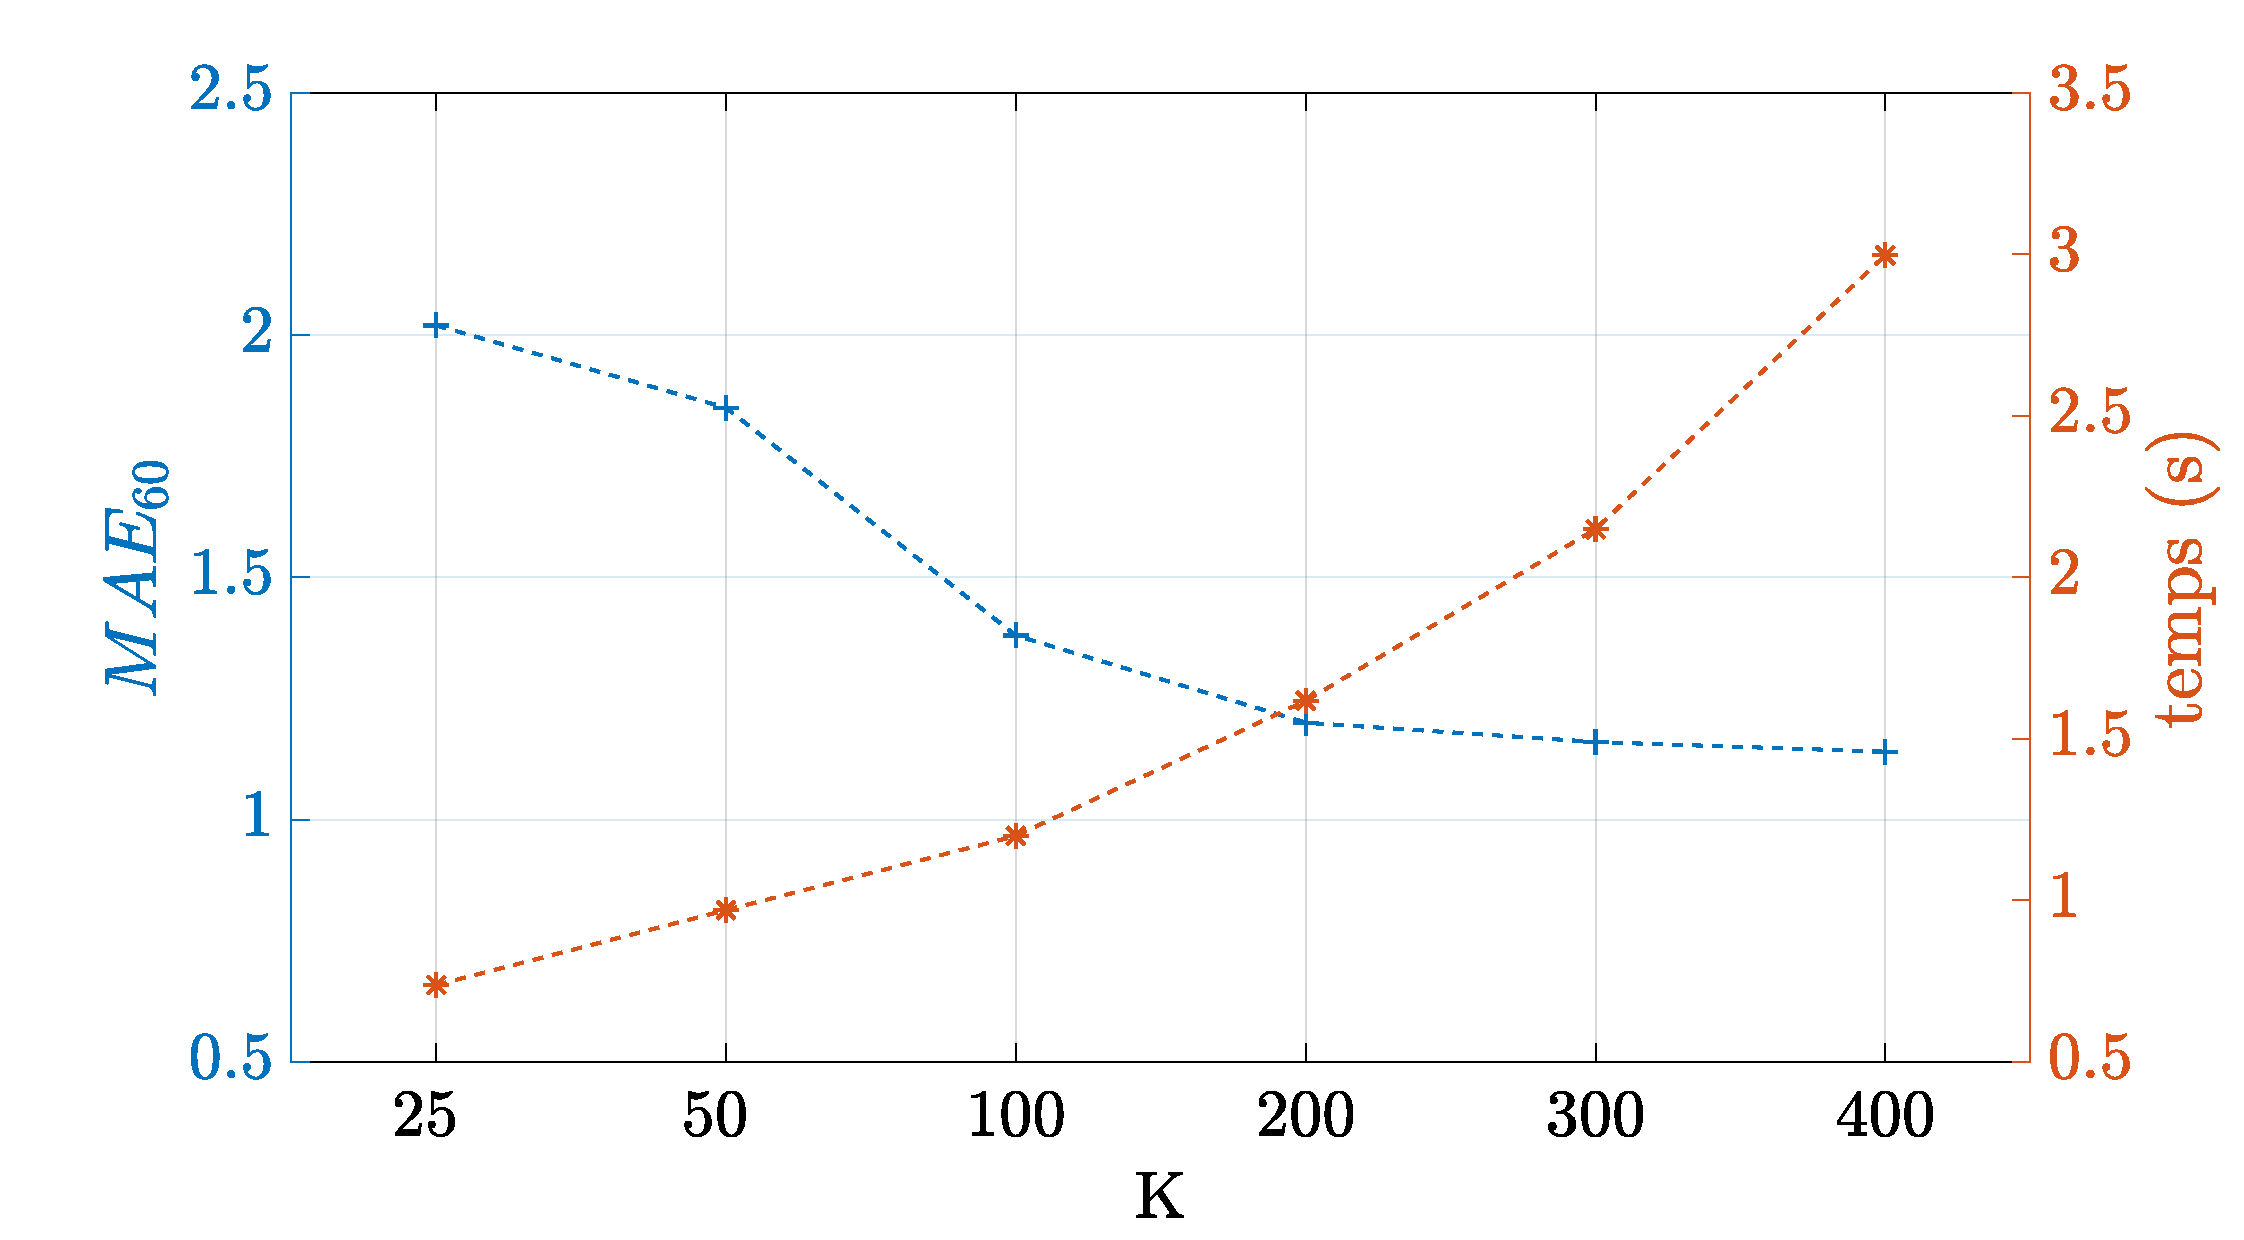
\includegraphics[width=.7\linewidth]{./figures/resultats/timeErrorNMF_IS_K.pdf}
\caption{Évolution de l'erreur $MAE_g$ et du temps de calcul selon la taille des matrices $K$.} 
\label{fig:errorTime}
\end{figure}

Cette durée reste cependant faible au regard des utilisations qui peuvent être faites de cette outil : en effet pour la réalisation de cartes de bruit ou la prédiction du bruit de trafic en milieu urbain, connaitre avec une grande précision, c'est-à-dire à la seconde par exemple, le niveau du trafic, n'a pas d'intérêt puisque les environnements sont habituellements caractérisés à des échelles temporelles grandes. \cite{broccoline} montre par exemple que 15 minutes sont nécessaires pour captuer les effets perceptifs d'un ESU. Dans le cas de la cartographie, leur mises à jour pour réaliser du temps réels sont souvent réalisés tout les heures \cite{} ou les quarts d'heure \cite{wei2016dynamic}. De plus, dans le cas où la mesure a pour but d'améliorer les cartes de bruits via des méthodes d'assimilations de données, cette génère un temps de calcul plus élevé qui rend donc la durée de l'estimation du niveau sonore par la NMF IS satisfaisante et adéquate.

\section{Comparaison des niveaux sonores $L_{eq,tr.,1s}$ pour plusieurs scènes sonores.}

L'étude des scènes sonores urbaines et l'estimation de leurs niveaux sonores du trafic a été réalisée sur un temps d'intégration de 1 minute pour le corpus \textit{SOUR}. 
Si la NMF IS optimale ($\beta$ = 2, $K$= 300, $w_t$ = 1, $t_h$ = 0,35) offre la meilleure estimation du $L_{eq,tr.,60s}$ sur l'intégralité du corpus, il est intéressant de visualiser la qualité de la reconstruction du signal \textit{trafic} à une échelle plus réduite. En conséquence, l'évolution du niveau sonore $\tilde{L}_{eq,tr.,1s}$ de 4 scènes issues de chaque ambiance sonore est représenté. Ce niveau sonore est comparé au niveau sonore exact, $L_{eq,tr.,1s}$ ainsi qu'au niveau sonore obtenu par l'estimateur \textit{baseline} à $f_c$ = 500 Hz. L'évolution du niveau sonore de la classe de son \textit{interférante} ($L_{eq,int.}$) est également ajoutée. Les extraits sont choisis pour être représentatif du comportement général observé sur les autres scènes.
Dans un premier, les 60 premières secondes de la scène 7 de l'ambiance \textit{Parc} (qui correspond à la réplication de l'enregistrement 2-WE-03, voir Tableau \ref{tab:correspondance_parc} en annexe \ref{annexe:correspondanceNameSour}) sont observées en Figure \ref{fig:Lp_parc}.


\begin{figure}[h!]
\centering
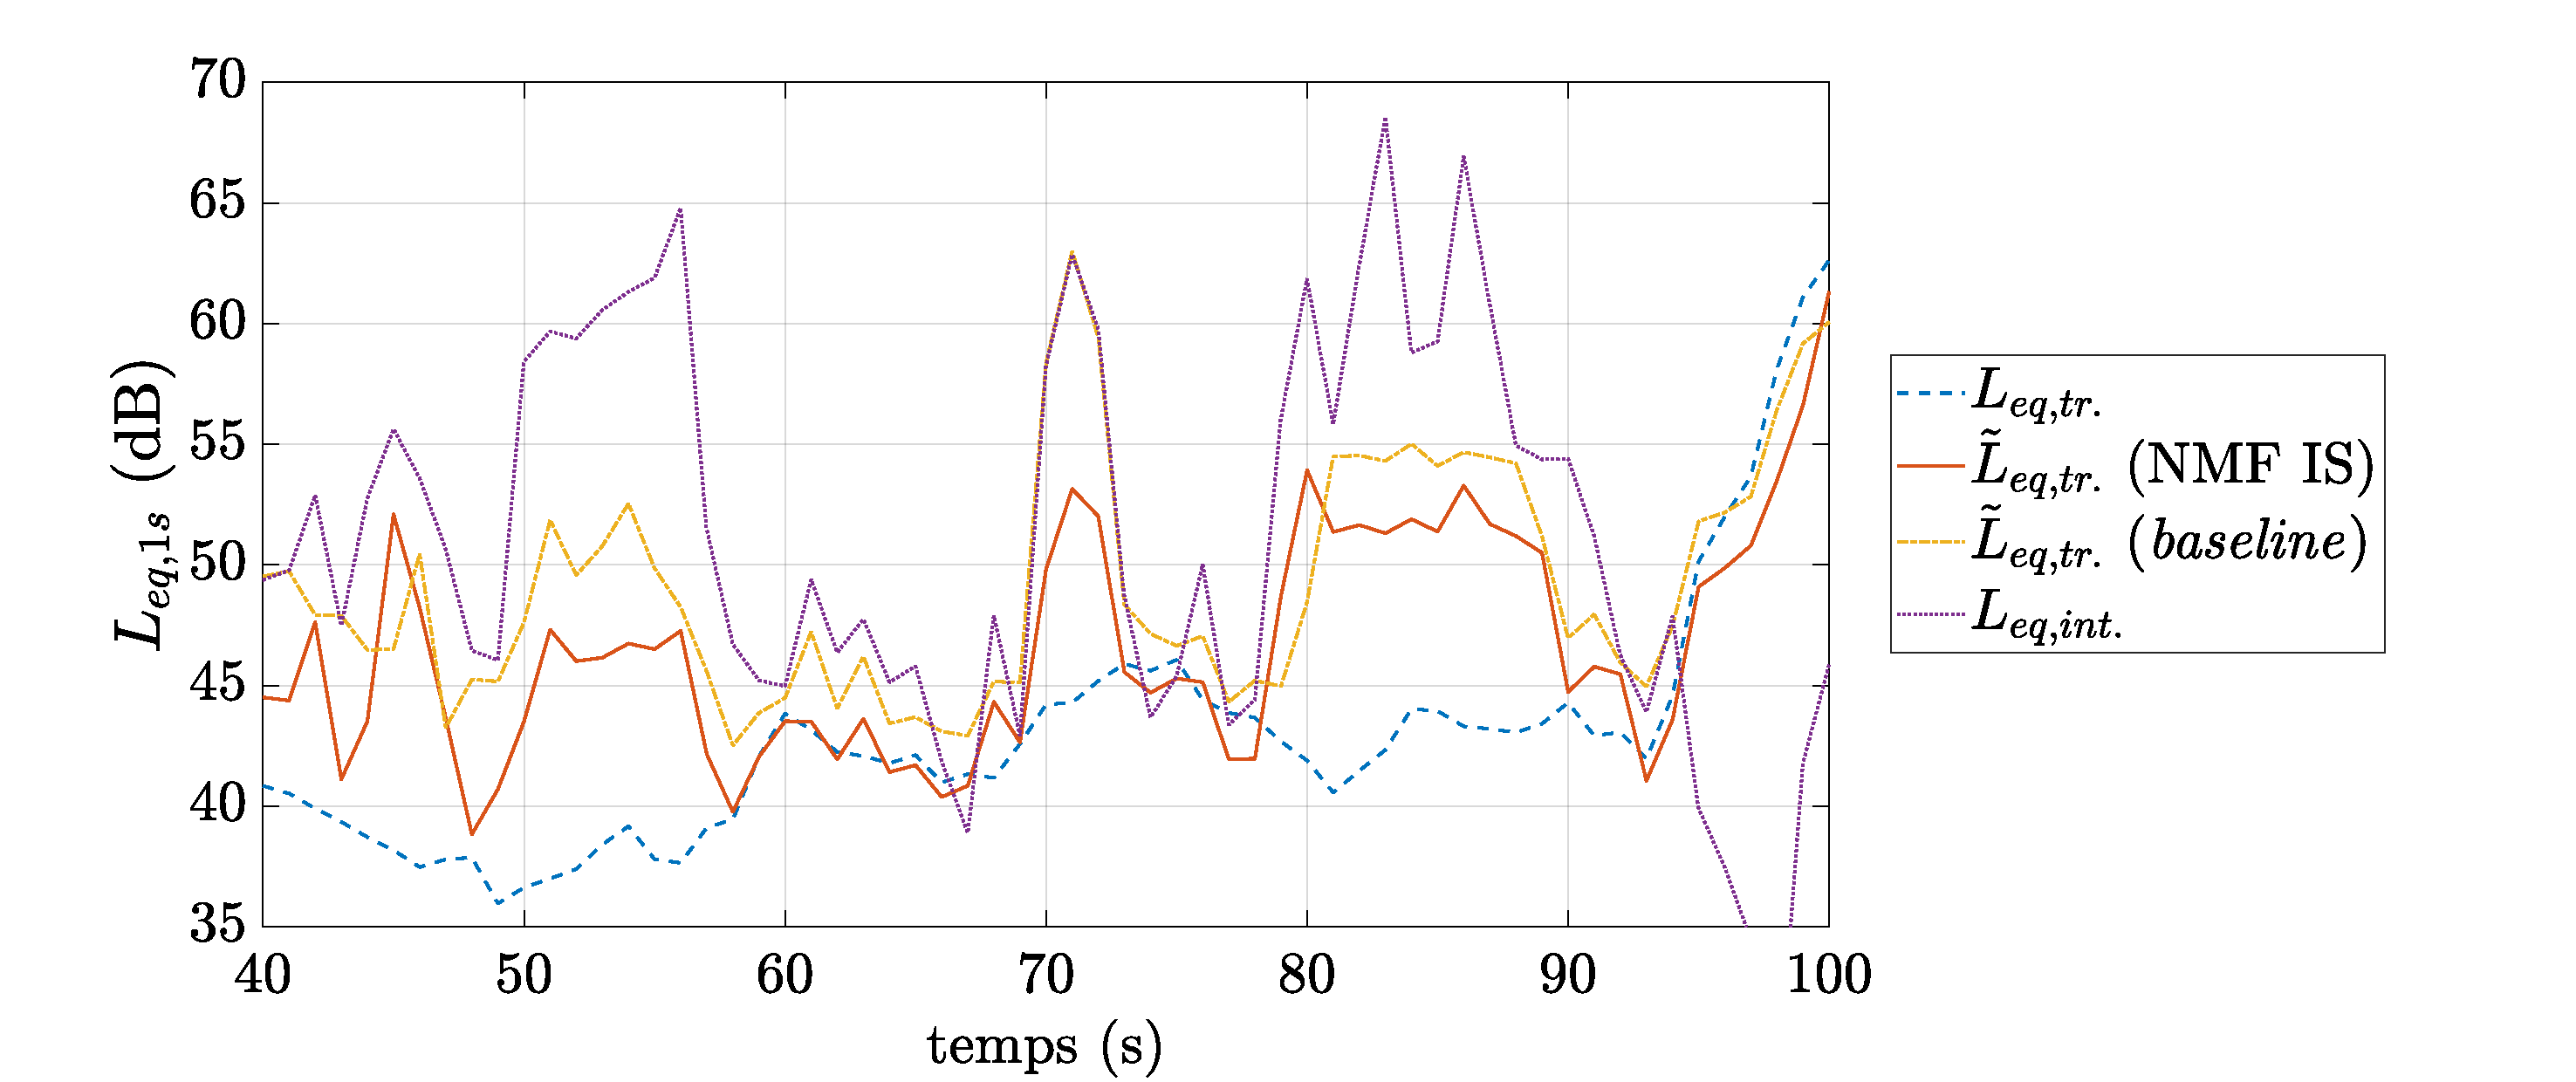
\includegraphics[width=.8\linewidth]{./figures/NMF/Lp_park_7.pdf} 
\caption{Évolution du niveau sonore équivalent $L_{eq, 1s}$ durant 60 secondes de la scène \textit{parc-07}.} 
\label{fig:Lp_parc}
\end{figure}

Cet extrait est notamment composé de trois bruits de fond (\textit{brouhaha parc}, \textit{oiseaux}, \textit{trafic routier})et est dominé par la classe de son interférante. 
L'erreur $MAE_{60}$ de l'estimateur NMF est de XX alors que celle de l'estimateur \textit{baseline} est de YY. 

On constate que cette erreur, pour les deux méthodes, est due à la classe interférante qui est modélisée par les estimateurs comme un signal \textit{trafic}. La NMF réussit alors à moins réaliser cette confusion, notamment dans les intervalles $\left[ 9,~20 \right]$ secondes, $\left[ 29,~33 \right]$ secondes et $\left[ 38,~50 \right]$ secondes qui correspondent respectivement à l'émergence d'un son de roulement de valise, d'un bruit de rue (barrière) et, successivement, d'un roulement de valise et de voix. L'estimation du niveaux sonore par la \textit{baseline} suit beaucoup plus la classe interférante que la NMF IS. 

\begin{figure}[h!]
\centering
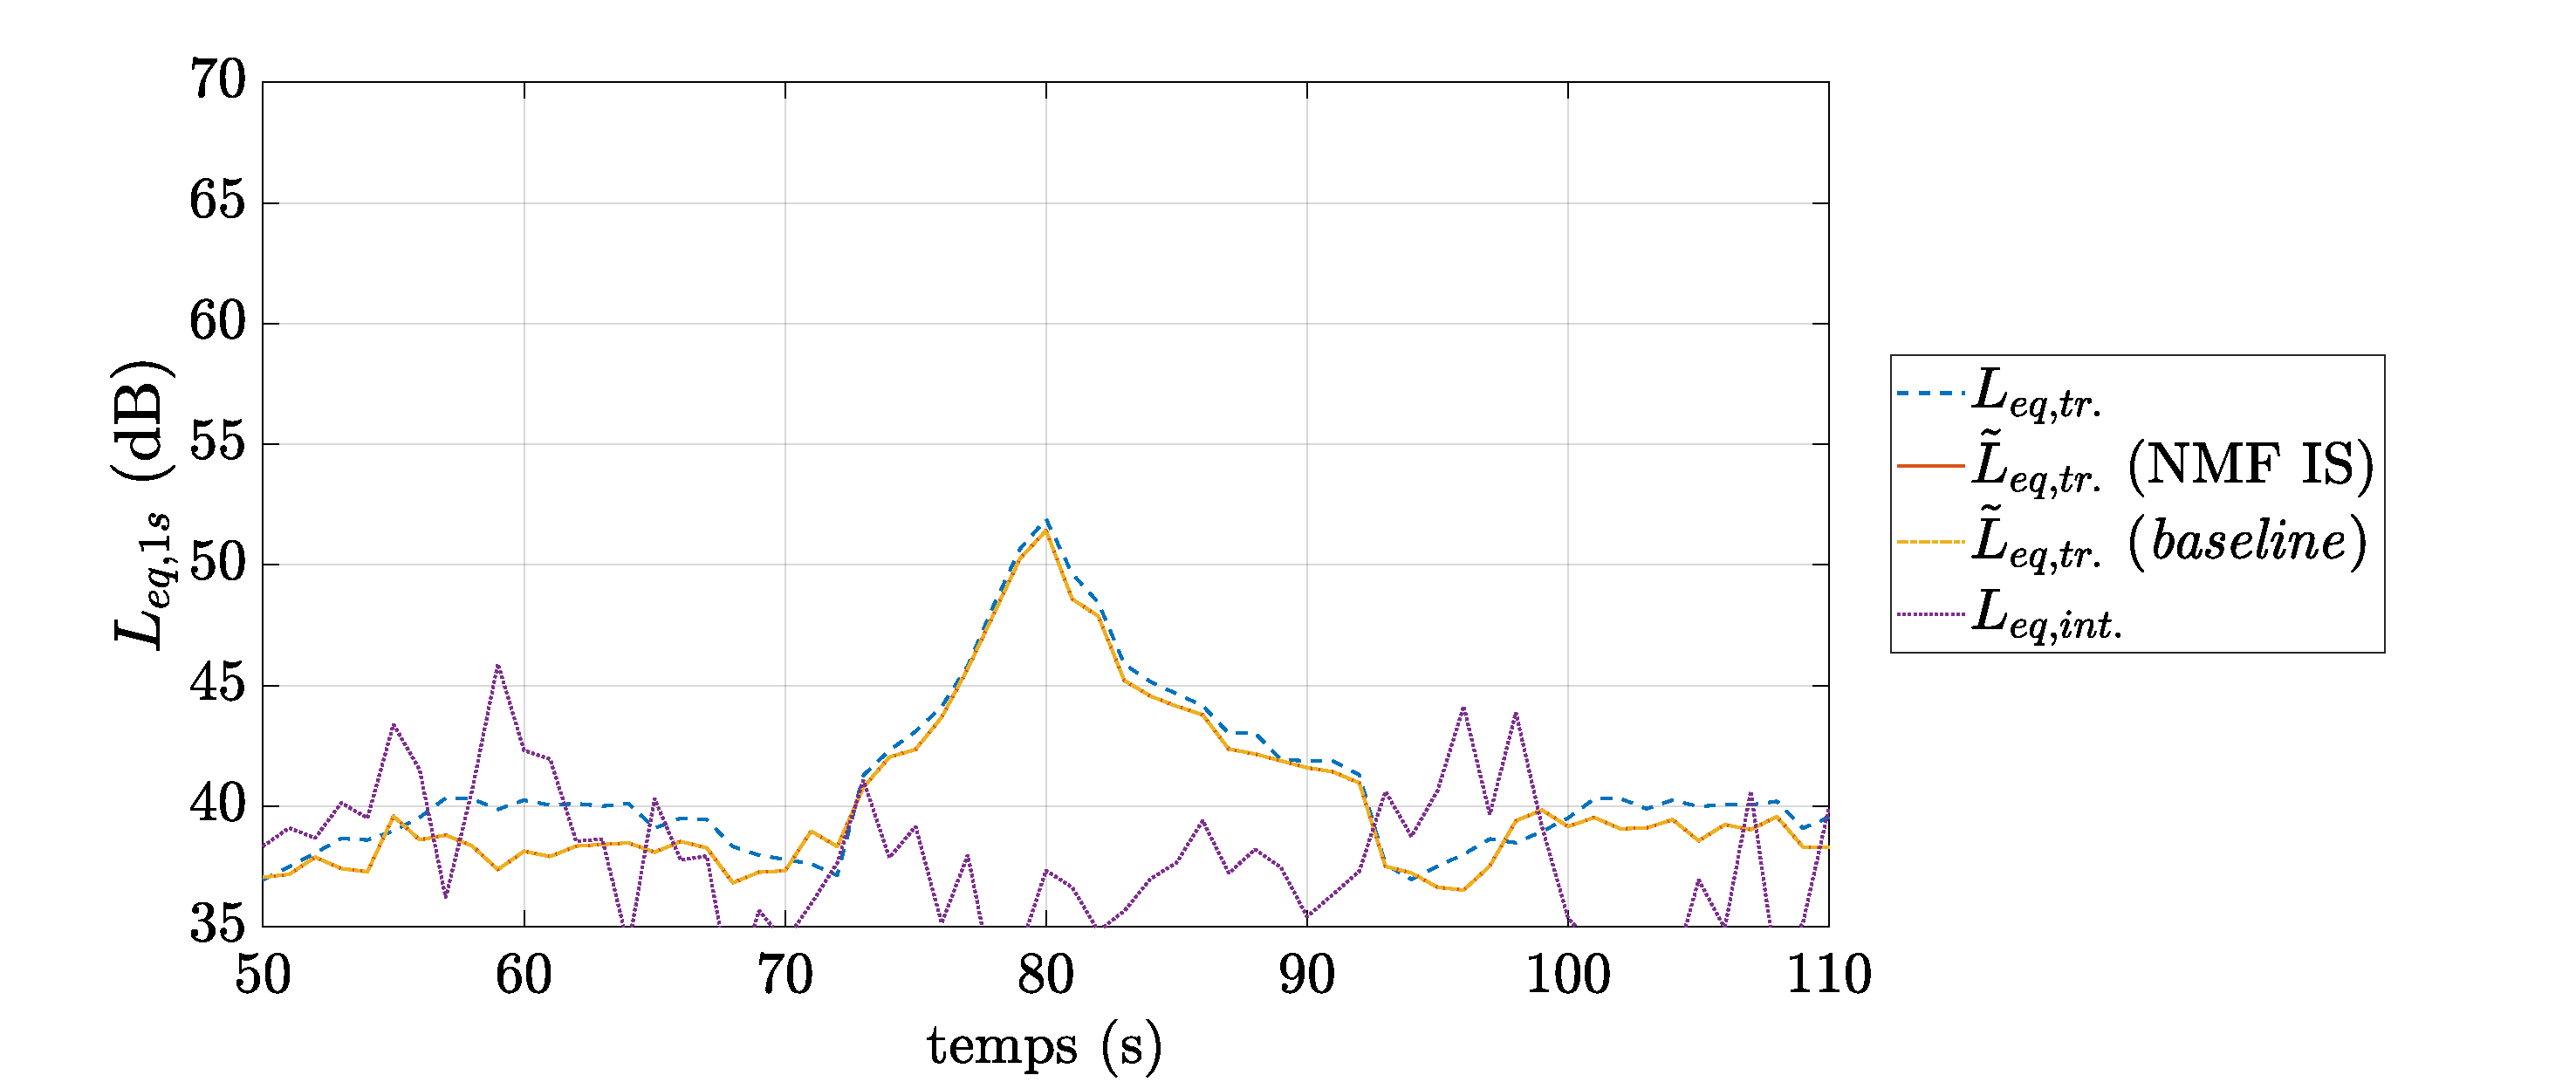
\includegraphics[width=.8\linewidth]{./figures/NMF/Lp_quietStreet_7.pdf} 
\caption{Évolution du niveau sonore équivalent $L_{eq, 1s}$ durant 60 secondes de la scène \textit{Rue Calme-07}.} 
\label{fig:Lp_quiet}
\end{figure}

La seconde scène observée en Figure \ref{fig:Lp_quiet} équivaut à un extrait de 1 minute de la 7\ieme{} scène de l'ambiance \textit{rue calme} (respectivement la réplication de  l'enregistrement 1-EW-17) entre la 50\ieme{} et la 110\ieme{} seconde. Elle se compose d'un bruit de fond \textit{oiseaux} et \textit{trafic} et d'évènements \textit{voix} ainsi que d'un passage d'une voiture entre la 70\ieme{} et la 93\ieme{} seconde. On observe que les deux estimateurs arrivent à bien estimer l'évolution du $L_{eq,tr.,1s}$ du passage du véhicule. En dehors de cet évènement, les deux estimateurs sont moins soumis à la classe interférante. L'erreur est alors due à une sous-estimation du niveau sonore \textit{trafic} qui est plus important pour la baseline.


\begin{figure}[h!]
\centering
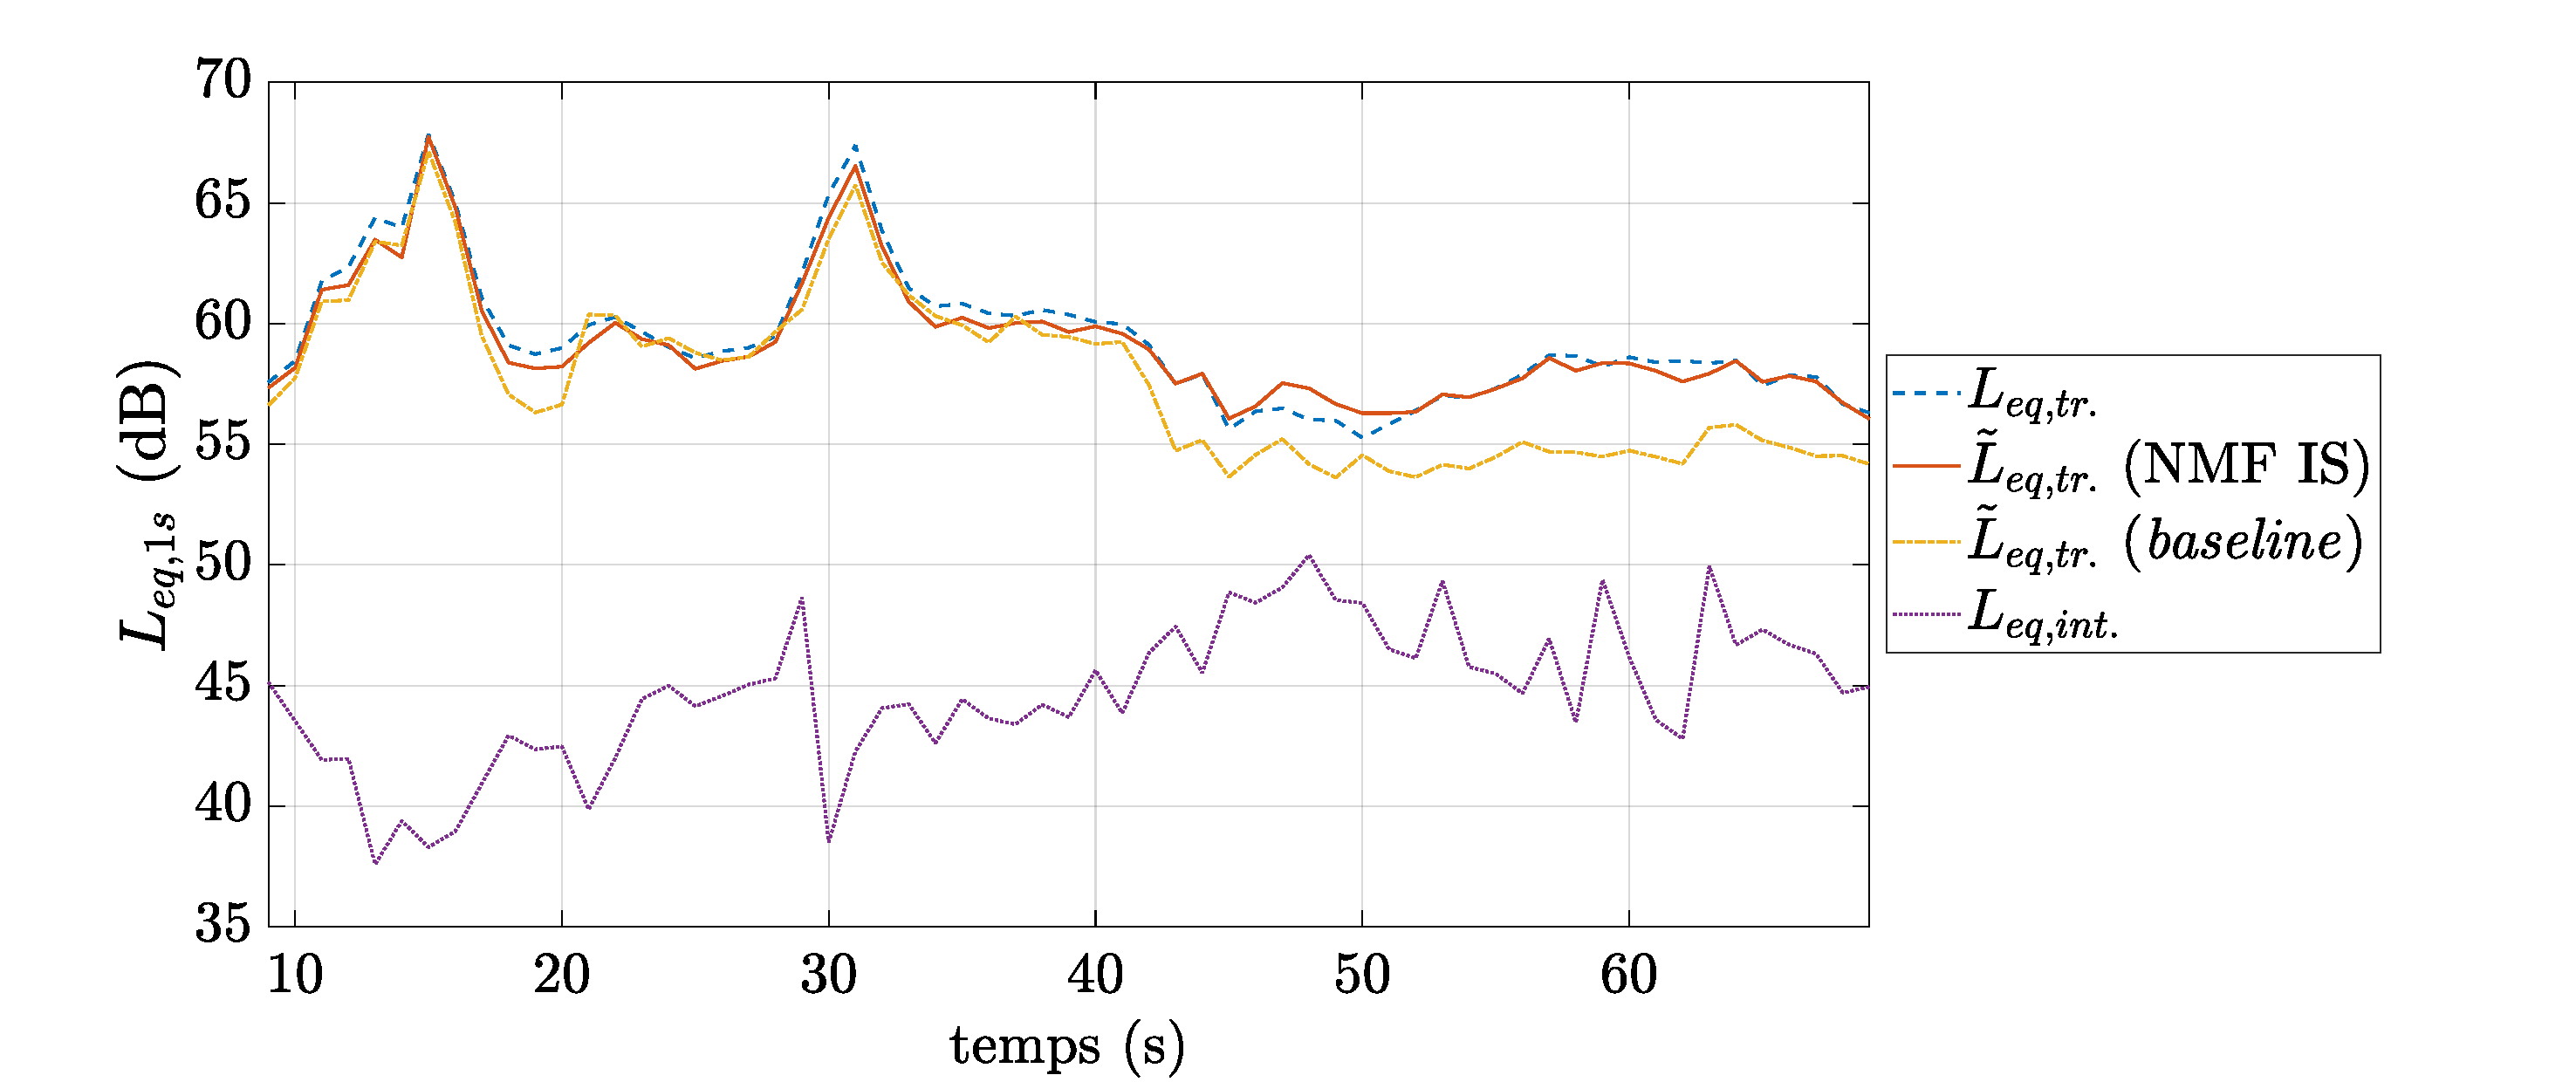
\includegraphics[width=.8\linewidth]{./figures/NMF/Lp_noisyStreet_3.pdf} 
\caption{Évolution du niveau sonore équivalent $L_{eq, 1s}$ durant 60 secondes de la scène \textit{Rue Bruyante-03}.} 
\label{fig:Lp_noisy}
\end{figure}

\begin{figure}[h!]
\centering
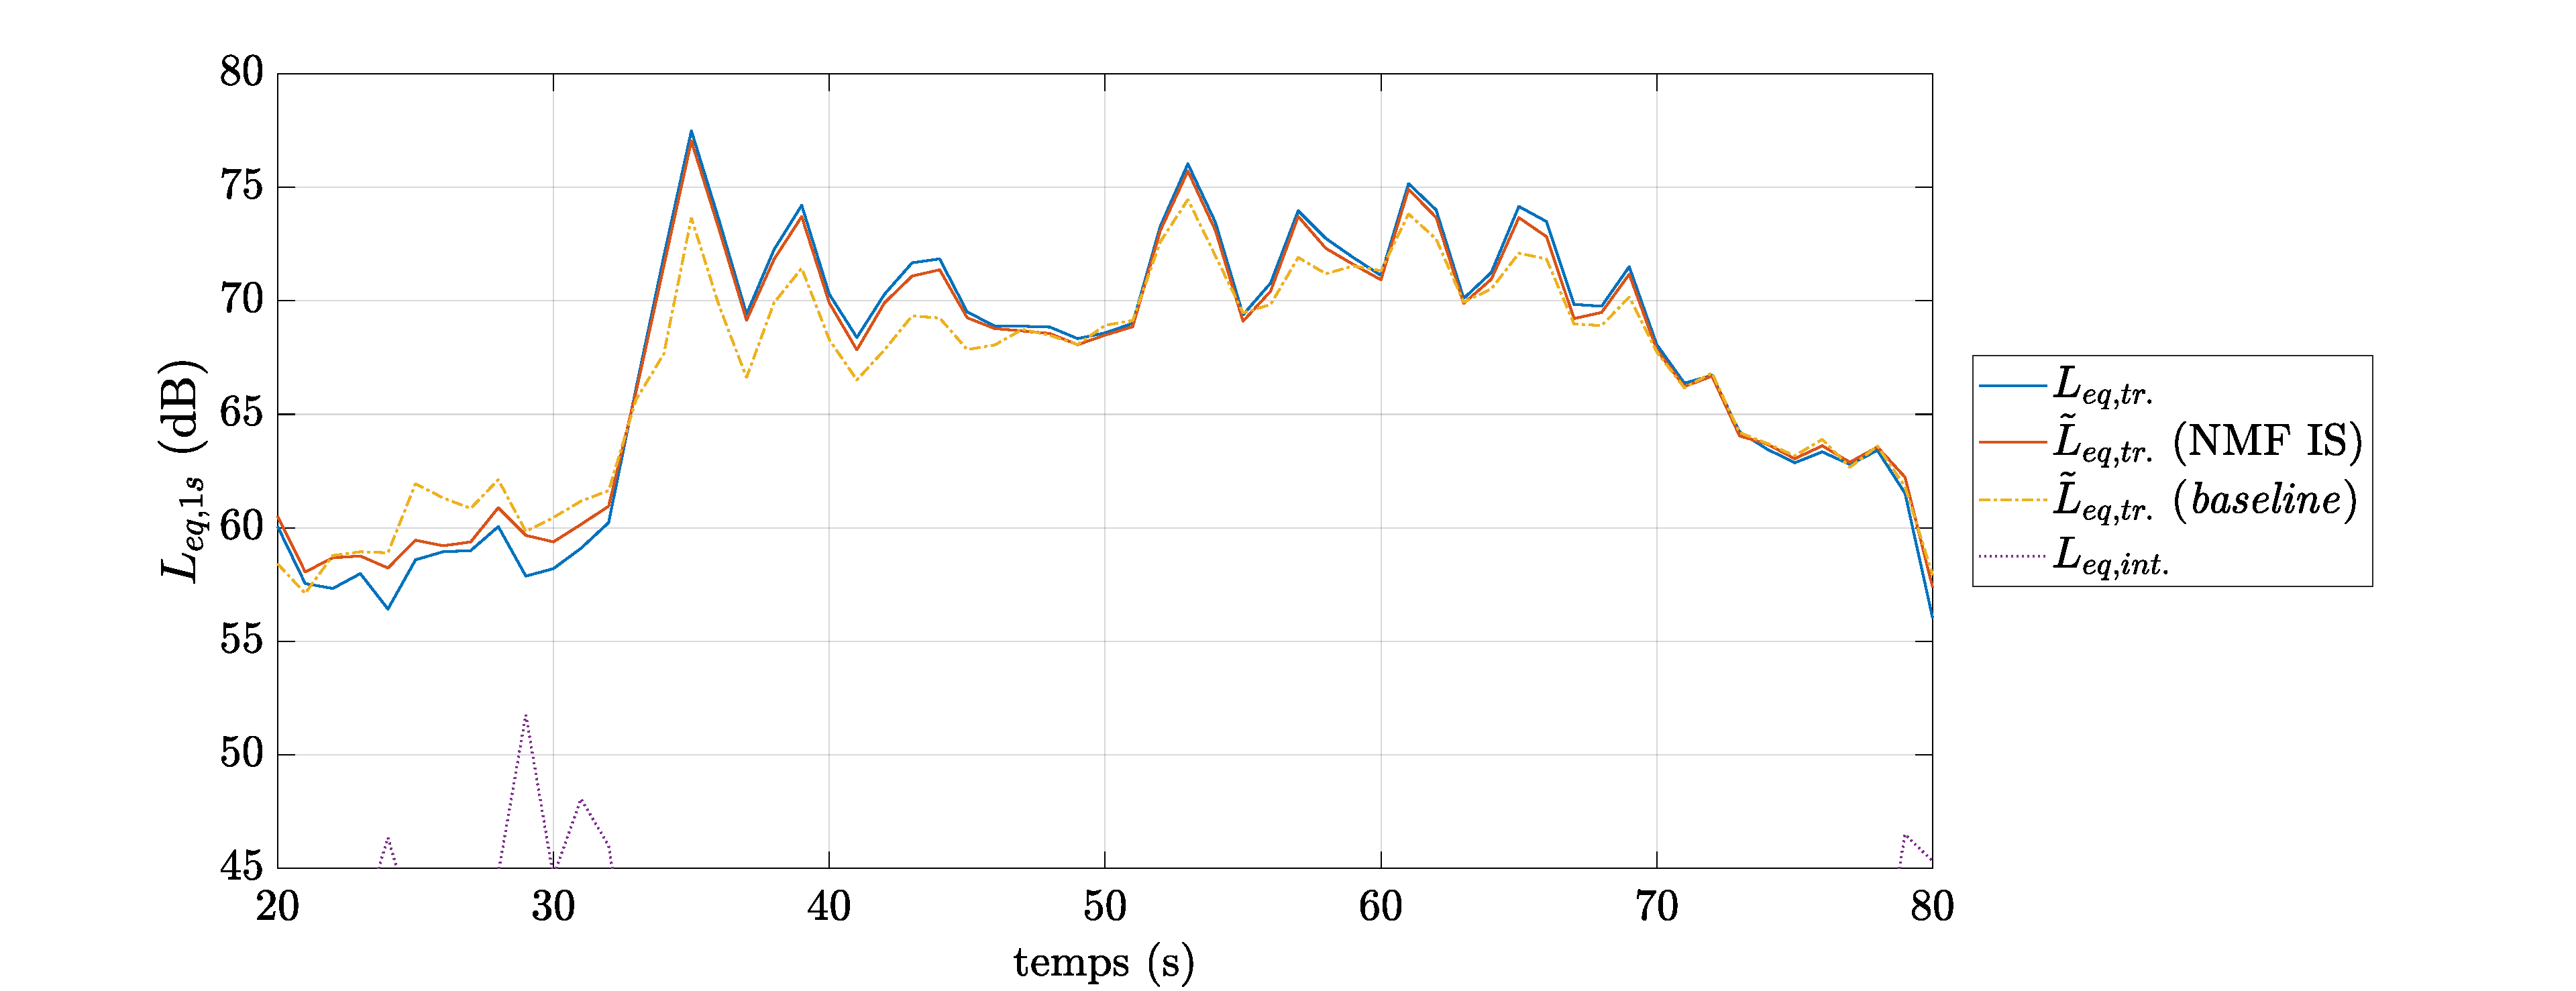
\includegraphics[width=.8\linewidth]{./figures/NMF/Lp_veryNoisyStreet_5.pdf} 
\caption{Évolution du niveau sonore équivalent $L_{eq, 1s}$ durant 60 secondes de la scène \textit{Rue Très Bruyante-05}.} 
\label{fig:Lp_veryNoisy}
\end{figure}


Les Figures \ref{fig:Lp_noisy} et \ref{fig:Lp_veryNoisy} résument des extraits des scènes \textit{bruyante-07} et \textit{très bruyante-05} (respectivement les répliques des enregistrements 01-EW-06 et 02-EW-16) où le trafic est la source sonore prédominante. L'extrait sonore de la Figure \ref{fig:Lp_noisy} est composé d'un bruit de fond de trafic ainsi que de voix en continu et d'oiseaux. Les évènements sonores appartiennent principalement à la classe \textit{trafic}. Malgré cela, si les passages des véhicules émergents entre la 10\ieme{} et la 40\ieme{} seconde sont correctement modélisés par les deux estimateurs, la NMF IS arrive ensuite beaucoup mieux à reconstruire le signal \textit{trafic} jusqu'à la fin de l'extrait que la baseline. Dans le cas de l'extrait sonore de la Figure \ref{fig:Lp_veryNoisy}, la classe de son \textit{interférante} composé de voix est très faible par rapport à la classe de son \textit{trafic}. Sur l'intervalle $\left[ 33,~72 \right]$ secondes, les multiples passages de voitures sont correctement estimés par la NMF IS. Si l'estimateur \textit{baseline} suit également cet évolution, il en estime toutefois les niveaux sonores.

En conclusion, les erreurs produites par les estimateurs, dans les ambiances \textit{Parc} et \textit{Rue Calme}, sont le plus souvent dues à la prise en compte de la composante \textit{interférante} dans le signal \textit{trafic}. Cette confusion est alors limitée par la NMF IS. Pour les ambiances \textit{Rue Bruyante} et \textit{Rue très bruyante}, l'estimateur baseline est notamment due à une sous estimation du niveau sonore en raison du rejet d'une partie de l'énergie sonore par le filtre passe-bas. 

\section{Pistes d'amélioration}

\`A partir de ces résultats, plusieurs pistes peuvent être envisagées pour améliorer l'estimation du niveau sonore du trafic. Parmi elles, l'ajout de la contrainte de régularité temporelle sur les activateurs est testé.

\subsection{Contrainte de régularité temporelle}

Cette contrainte, présentée dans la partie \ref{part:smoothness}, consiste à forcer les activateurs temporelles de la matrice $\mathbf{H}$ à adopter des variations plus lentes entre les trames temporelles. Son utilisation est justifié ici par le comportement de la source d'intérêt : le passage d'une voiture est un évènement qui a une durée de plusieurs secondes. En forçant les activateurs à adopter des variations plus lentes, on serait susceptible de pouvoir mieux modéliser cette source. Cette contrainte se traduit par l'ajout d'un second terme à la fonction de coût, 


\begin{equation}
\underset{\textbf{W},\textbf{H}}{\text{min}}~D\left(\textbf{V} \vert\vert \textbf{WH}\right) + \alpha_t C_t(\mathbf{H}),
\end{equation}


avec la contrainte de régularité temporelle $C_t(\mathbf{H})$ présentée dans la partie \ref{part:smoothness} par l'équation \ref{eq:smoothnessVirtanen} et rappelée ici : 

\begin{equation}
C_t(\mathbf{H}) = \sum_{n=1}^K \alpha_k\sum_{n=2}^N \left(h_{kn} - h_{k(n-1)}\right)^2,
\end{equation}

et la pondération $\alpha_t$ qui modifie l'importante de cette contrainte dans la mise à jour de la matrice $\mathbf{H}$.
Cette contrainte s'applique sur les trois versions de la  NMF testées. Dans les cas de la NMF SUP et le NMF IS, cette contrainte s'applique sur l'ensemble des matrices $\mathbf{H}$ puisqu'elles sont composées dans entièrement de spectres \textit{trafic}. Leur mises à jour suivent donc l'équation \ref{eq:HupdateSmooth}. Dans le cas de la NMF SEM, le dictionnaire se décompose en deux parties (une partie fixe $\mathbf{W_s}$ composée de spectres \textit{trafic} et une partie libre $\mathbf{W_r}$). Pour favoriser les variations lentes des activateurs temporelles des spectres \textit{trafic}, cette contrainte est seulement posée pour $\mathbf{H_s}$. La mise à jour de la matrice suit donc l'équation \ref{eq:HupdateSmooth} alors que celle de $\mathbf{H_r}$ reste la même (équation \ref{eq:HupdateMM}).
La pondération $\alpha$ est définie pour plusieurs valeurs : $\alpha_t \in \lbrace 0,01,~ 0,05,~ 0,1,~ 0,5,~ 1,~2,~3,~5 \rbrace$ testé pour l'association des différentes modalités des facteurs expérimentaux présentés dans la partie \ref{part:rappelExp}. 400 itérations sont ensuite réalisées.
L'augmentation du nombre d'itération est nécessaire afin d'obtenir une convergence satisfaisante des fonctions de coûts. L'impact de la contrainte sur la distance $D(\mathbf{V}\Vert \mathbf{WH})$ est observé pour une NMF SUP, SEM et IS. 
Dans le cas de la NMF SUP, cette contrainte permet la diminution de la fonction de coût. En contraignant les activations, les éléments \textit{trafic} sont alors moins susceptibles d'être activés pour modéliser la classe interférante. Dans le cas de la NMF SEM, cette contrainte génère une augmentation de la fonction de coût et également une convergence plus lente que sans contrainte. Après 400 itérations, celle-ci reste supérieure à celle sans pondération obtenue après 200 itérations. Sous la contrainte de régularité temporelle, la reconstruction globale du signal semble donc moins bonne.
 
\begin{figure}[h]
\centering
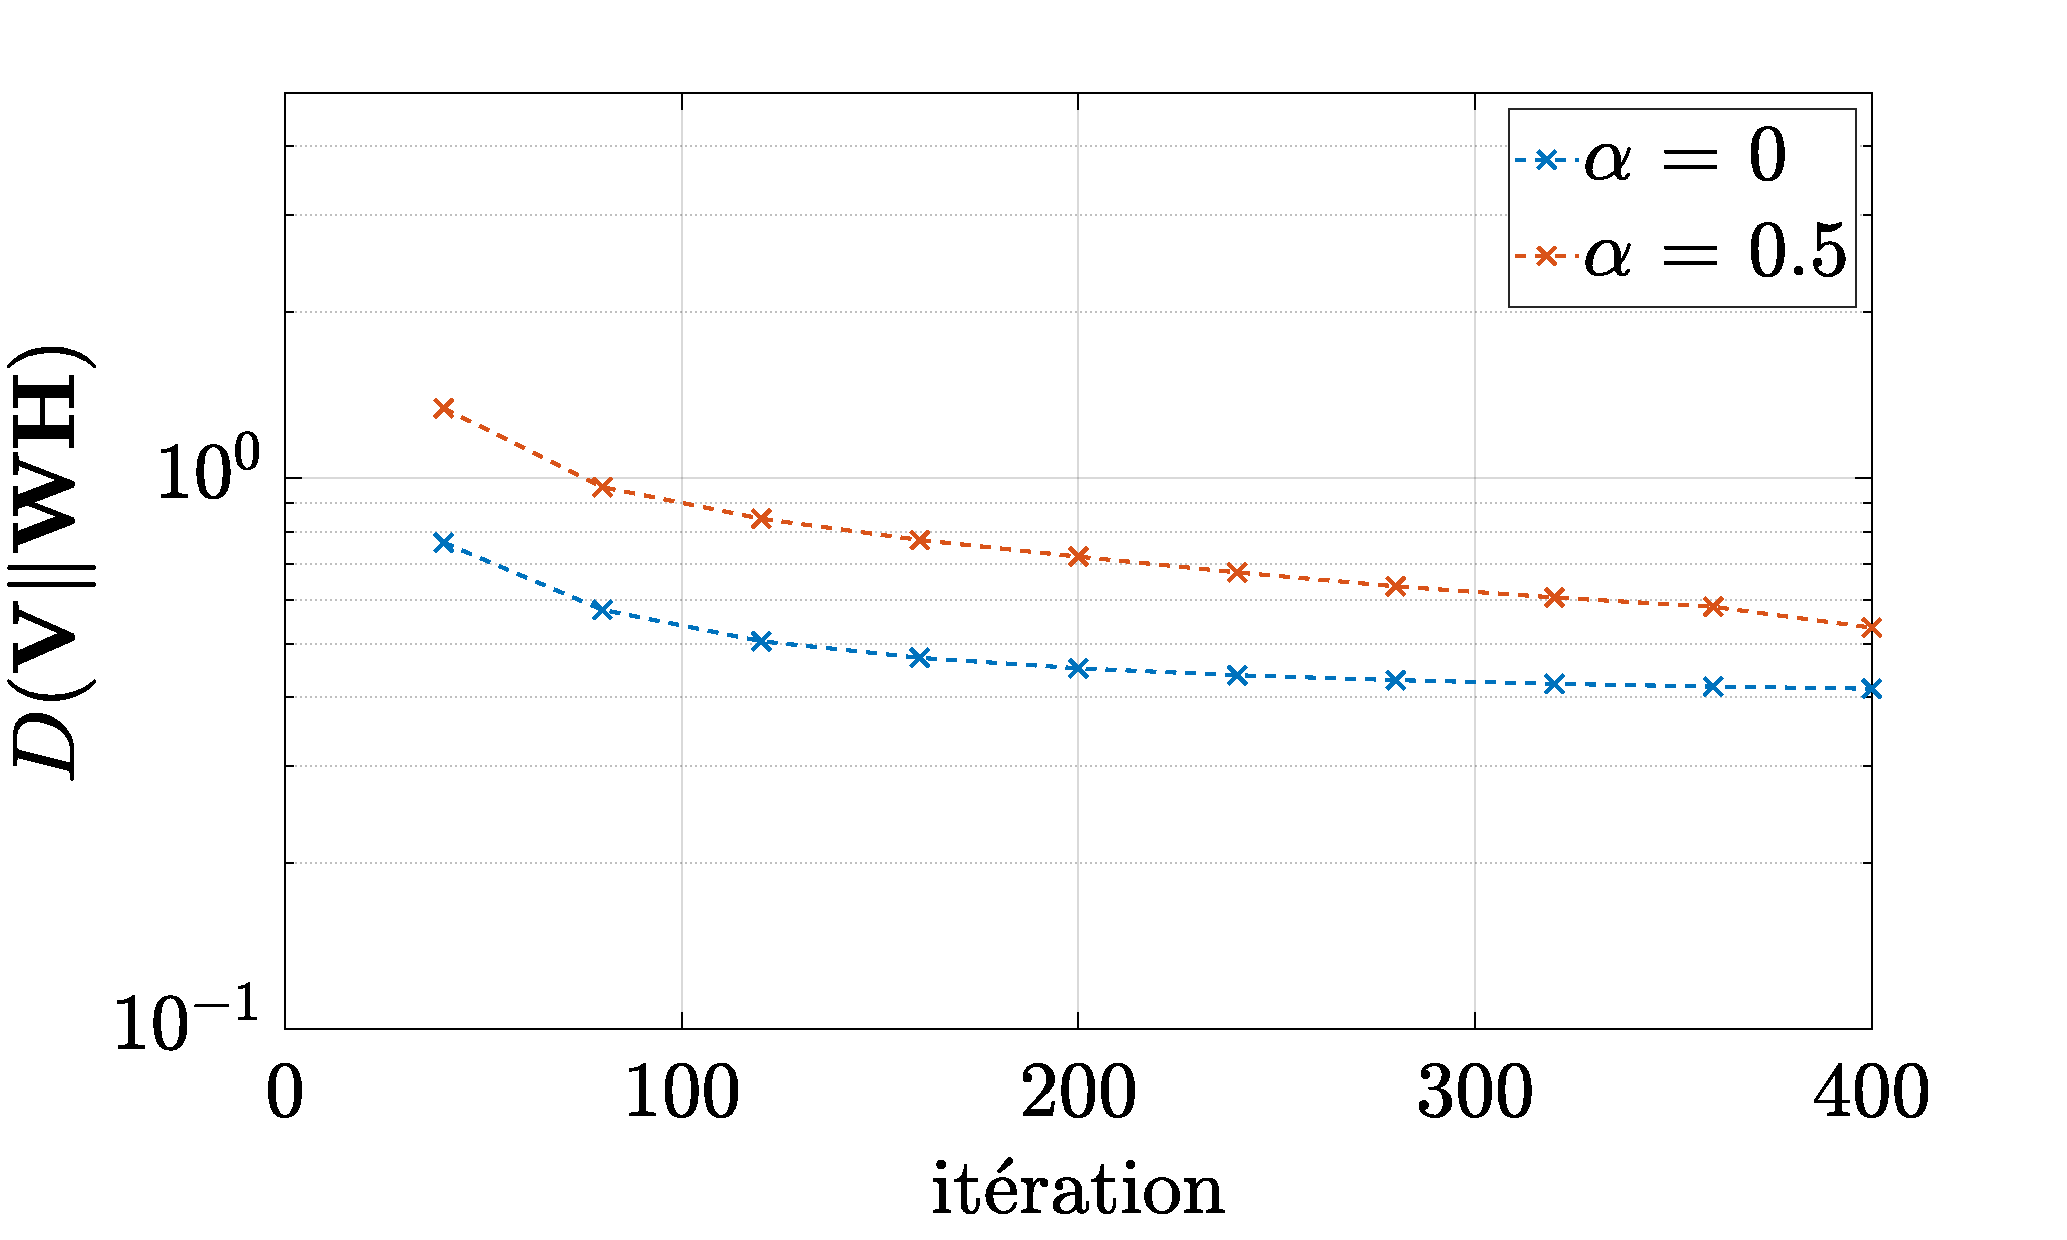
\includegraphics[width=.8\linewidth]{./figures/resultats/grafic_smooth_cost_beta0.pdf}
\caption{Influence de la régularité temporelle sur la fonction de coût pour la NMF SEM avec $\beta$ = 0, $w_t$ = 2 s et $K$ = 300.}
\end{figure}

\begin{table}[h!]
\centering
\caption{Erreurs $MAE_{60}$ pour les combinaisons optimales de modalités des estimateurs pour le corpus d'évaluation \textit{SOUR} en présence d'une pondération de régularité temporelle.}
\label{tab:erreur_smooth}
\resizebox{\textwidth}{!}{%
\begin{tabular}{L{2cm}C{1.5cm}C{1.2cm}C{1.2cm}C{1.2cm}C{1.2cm}C{2.5cm}C{2.5cm}}
\toprule
méthode & $f_c$ (kHz) & $\beta$ & $w_t$ & K & $t_h$ & $\alpha$ & $MAE_{60}$ \\ \toprule
\multirow{2}{*}{filtre PB} & 20 & - & - & - & - & - & 3,62 ($\pm$ 3,93) \\
 & 0,5 & - & - & - & - & - & 1,99 ($\pm$ 1,37) \\ \midrule
\multirow{3}{*}{NMF SUP}  & - & 2 & 0,5 & 25 & - & - & 2,13 ($\pm$ 2,22) \\ 
 & - & 0 & 0,5 & 200 & - & 2 & 3,54 ($\pm$ 3,75) \\
 & - & 1 & 0,5 & 200 & - & 3 & 2,56 ($\pm$ 2,58) \\
 & - & 2 & 0,5 & 25 & - & 0,01 & 2,12 ($\pm$ 2,14) \\ \midrule
\multirow{3}{*}{NMF SEM}  & - & 1 & 0,5 & 300 & - & - &  1,93 ($\pm$ 0,42) \\
 & - & 0 & 2 & 300 & - & 0,5 & 1,53 ($\pm$ 0,81) \\
 & - & 1 & 0,5 & 300 & - & 0,5 &  1,84 ($\pm$ 0,34) \\
 & - & 2 & 2 & 300 & - & 5e-3 & 2,19 ($\pm$ 0,61) \\ \midrule
\multirow{3}{*}{NMF IS}  & - & 2 & 1 & 300 & 0,35 & - & 1,16 ($\pm$ 0,86) \\
 & - & 0 & 50 & 0 & 1 & 0,44 & 1,66 ($\pm$ 1,14) \\
 & - & 1 & 1 & 200 & 0,35 & 0,36 & 1,37 ($\pm$ 0,76) \\
 & - & 2 & 1 & 300 & 0,35 & 0,34 & 1,48 ($\pm$ 0,90) \\
 \bottomrule
\end{tabular}}
\end{table}

Toutefois, la qualité de la reconstruction global du signal ne signifie pas que celle de la composante \textit{trafic} soit incorrect. Pour cela, les erreurs $MAE_g$ minimales obtenues avec la NMF SUP, SEM et IS pour chaque valeur de $\beta$ en fonction de la valeur de la pondération sont résumées dans le Tableau \ref{tab:erreur_smooth}. Les erreurs minimales obtenues par chaque méthode dans la partie \ref{chap:grafic_nmf} sont également adjointes pour servir de référence.

L'ajout de la contrainte de \textit{smoothness} a un impact positif sur la NMF SUP pour $\beta \in \lbrace 1,~2 \rbrace$. Dans le cas de la divergence KL, cette contrainte génère un changement dans la composition du dictionnaire avec un faible nombre d'éléments. Cependant, dans le cas de la distance EUC, l'influence de la contrainte est trop faible pour pouvoir être considérée.

Dans le cas de la NMF SEM, l'influence de la pondération est positif pour la divergence KL et la divergence IS. Dans ce dernier cas, pour un dictionnaire de même taille (avec une fenêtre toutefois différente), la diminution est importante avec une erreur $MAE_g = 1,53$. 
Dans la Figure \ref{fig:smoothMAE60}, on compare la méthode optimale sans pondération ($\beta$ = 1, $K$ = 300, $w_t$ = ), la combinaison pour $\beta$ = 0 ($K$ = 300, $w_t$ = ) sans et avec pondération. 

La version optimale de la NMF SEM basée sur la divergence de KL présente une évolution des erreurs déjà observé précédemment : de plus fortes erreurs pour les ambiances \textit{Parc} et \textit{rue calme} qui diminue avec la prédominance du trafic routier. 
La NMF basé sur la divergence de IS, sans pondération, génère des erreurs différentes notamment dans l'ambiance \textit{parc} où l'erreur est beaucoup plus faible ($MAE_g$ = ). L'ajout de la contrainte de \textit{smoothness} détériore ces performances mais permet une meilleure estimation du signal \textit{trafic} pour les 3 autres ambiances sonores.
En conclusion, les degrés de liberté de la NMF SEM, s'ils permettent plus d'adaptabilité et de souplesse, gagne ici à être contraint afin de mieux se focaliser sur la source sonore \textit{trafic}. 

\begin{figure}[h!]
\centering
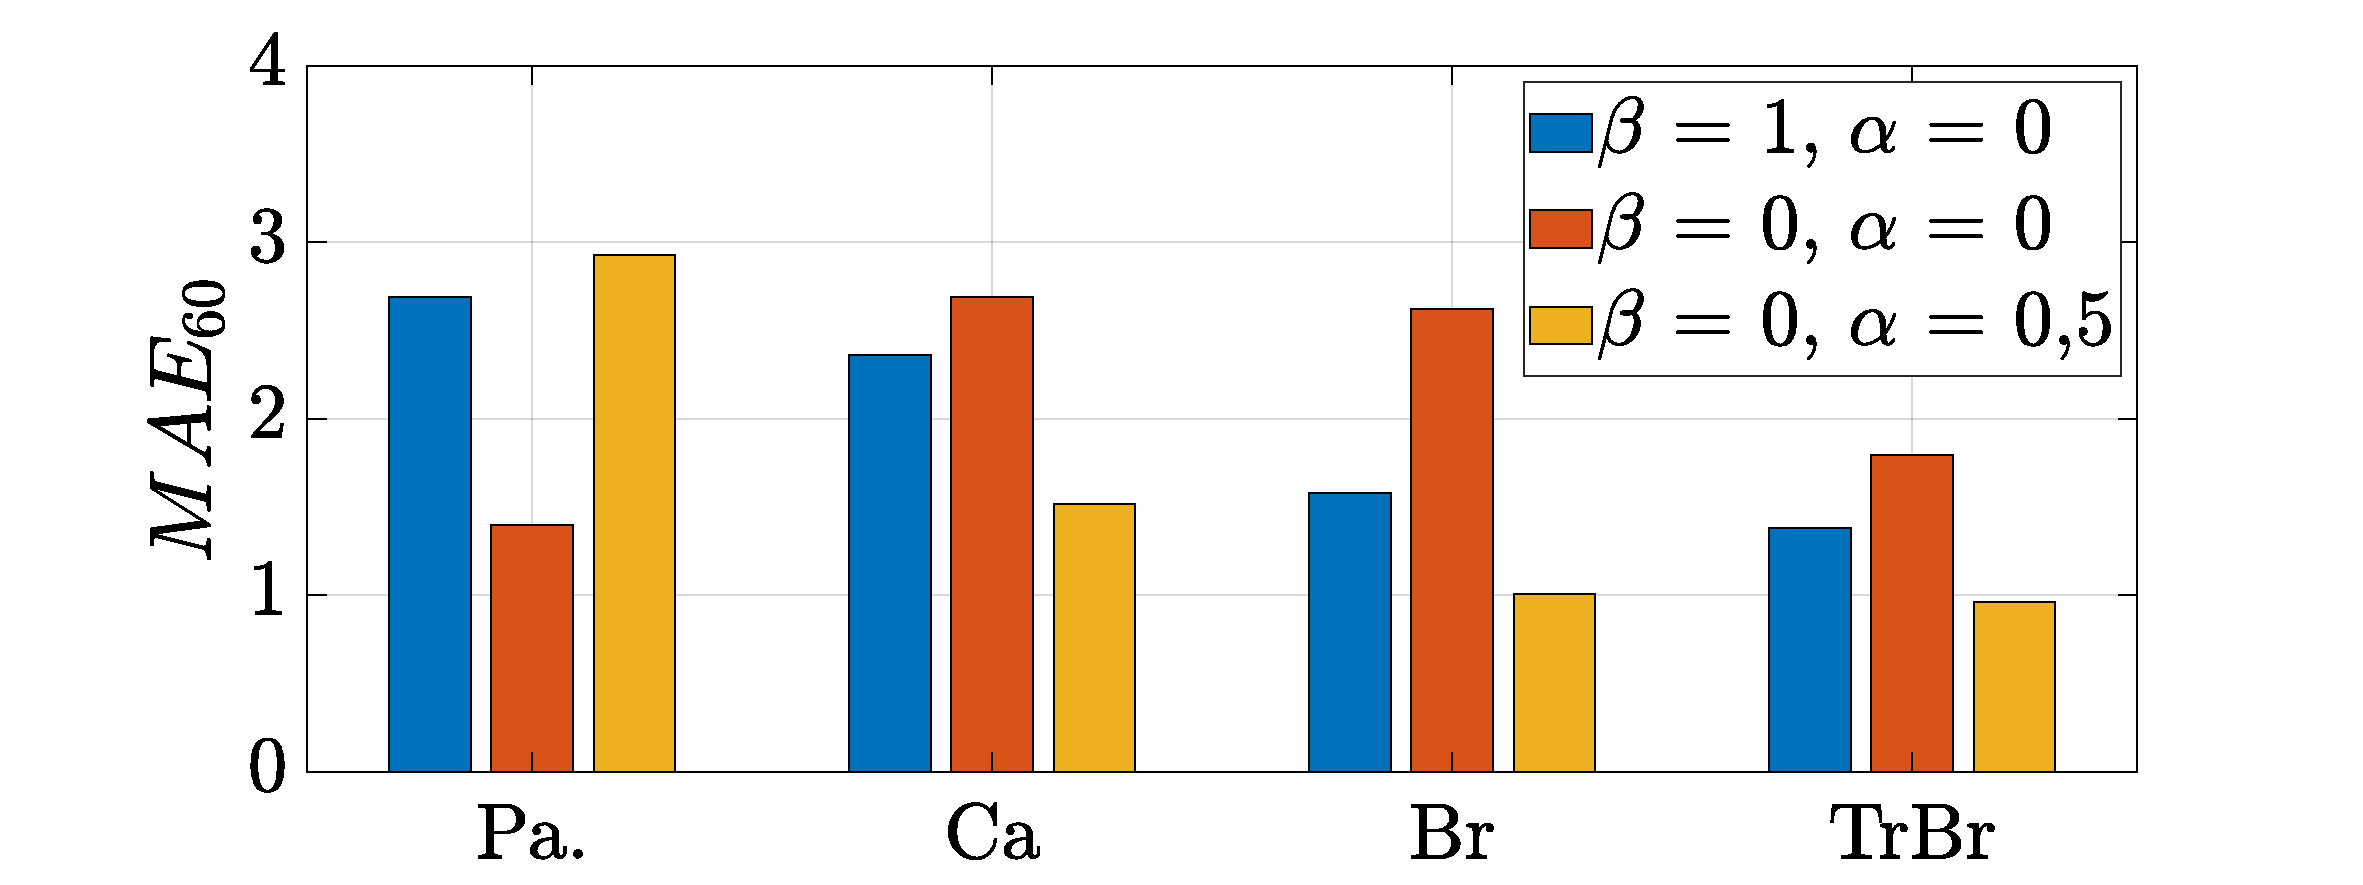
\includegraphics[width=.9\linewidth]{./figures/resultats/grafic_smooth_bar.pdf}
\caption{Influence de la pondération de régularité temporelle pour la NMF SEM selon chaque ambiance sonore.}
\label{fig:smoothMAE60}
\end{figure}


\subsection{Contrainte par parcimonie}

Une autre contrainte est maintenant considérée : la contrainte de parcimonie (ou \textit{sparsness}). Appliquée sur la matrice $\mathbf{H}$, celle-ci a pour but de réduire le nombre de base activée à chaque trame. Cette contrainte se présente comme la contrainte de \textit{smoothness} : 

\begin{equation}
\underset{\textbf{W},\textbf{H}}{\text{min}}~D\left(\textbf{V} \vert\vert \textbf{WH}\right) + \alpha_{sp} C_{sp}(\mathbf{H}).
\end{equation}

avec $C_{sp}(\mathbf{H})$, la contrainte exprimée dans l'équation \ref{eq:sparsness} et $\alpha_{sp}$ la pondération. De même que pour la contrainte de \textit{smoothness}, la parcimonie est appliqué sur les matrices $\mathbf{H}$ de la NMF SUP et IS. Pour la NMF SEM, cette contrainte est appliquée non pas sur $\mathbf{H_s}$ mais sur $\mathbf{H_r}$ afin de mieux inclure les évènements ponctuels dans $\mathbf{W_r}$ et moins les composantes \textit{trafic}. La parcimonie est testée pour plusieurs valeurs de pondération : $\alpha_{sp} \in \left[0.05 0.1 0.2 0.5 1\right]$. 400 itérations sont également réalisées sur l'ensemble des combinaisons testées. Le Tableau \ref{tab:erreur_sparse} résume les erreurs $MAE_g$.

\begin{table}[h!]
\centering
\caption{Erreurs $MAE_{60}$ pour les combinaisons optimales de modalités des estimateurs pour le corpus d'évaluation \textit{SOUR} en présence d'une pondération de parcimonie.}
\label{tab:erreur_sparse}
\begin{tabular}{L{2cm}C{1.5cm}C{1.2cm}C{1.2cm}C{1.2cm}C{1.2cm}C{2.5cm}C{2.5cm}}
\toprule
méthode & $f_c$ (kHz) & $\beta$ & $w_t$ & K & $t_h$ & $\alpha$ & $MAE_{60}$ \\ \toprule
\multirow{2}{*}{filtre PB} & 20 & - & - & - & - & - & 3,62 ($\pm$ 3,93) \\
 & 0,5 & - & - & - & - & - & 1,99 ($\pm$ 1,37) \\ \midrule
\multirow{3}{*}{NMF SUP}  & - & 2 & 0,5 & 25 & - & - & 2,13 ($\pm$ 2,22) \\ 
 & - & 0 & 0,5 & 200 & - & 0,5 & 3,73 ($\pm$ 4,01) \\
 & - & 1 & 0,5 & 50 & - & 0,05 & 2,50 ($\pm$ 1,90) \\
 & - & 2 &  &  & - &  & ($\pm$) \\ \midrule
\multirow{3}{*}{NMF SEM}  & - & 1 & 0,5 & 300 & - & - &  1,93 ($\pm$ 0,42) \\
 & - & 0 & 2 & 300 & - & 0,50 & 1,99 ($\pm$ 0,70) \\
 & - & 1 & 0,5 & 100 & - & 0,05 &  1,50 ($\pm$ 0,89) \\
 & - & 2 &  &  & - &  & ($\pm$) \\ \midrule
\multirow{3}{*}{NMF IS}  & - & 2 & 1 & 300 & 0,35 & - & 1,16 ($\pm$ 0,86) \\
 & - & 0 &  &  &  &  & ($\pm$) \\
 & - & 1 &  &  &  &  & ($\pm$) \\
 & - & 2 &  &  &  &  & ($\pm$) \\
 \bottomrule
\end{tabular}
\end{table}

\subsection{Optimisation par les environnements sonores}\label{part:optimisationESU}


La NMF IS optimale trouvée dans la partie \ref{chap:grafic_nmf} ($\beta$ = 2, $K$ = 300 et $w_t$ = 1 s) est définie selon un seuil fixe sur l'ensemble du corpus et des ambiances sonores. Toutefois, il peut être possible de diminuer ces erreurs en adaptant le seuil $t_h$ à chaque environnement sonore. 
Cette adaptation peut être facilement mise en place pour les réseaux de capteurs fixes par l'estimation de l'ESU aux alentours du microphone. Une fois celui-ci le seuil correspondant à l'ambiance sonore est choisie. 
En considérant la NMF IS optimale avec $\beta$ = 2, $K$ = 300 et $w_t$ = 1 s, les seuils optimaux $t_{h,opt.}$ et les erreurs $MAE_{60}$ correspondantes par ambiance sont résumées dans le Tableau \ref{tab:erreur_optimise}.

\begin{table}[h]
\centering
\caption{Erreurs $MAE_{60}$ minimales selon le seuil optimal $t_{h,opt}$ par ambiance sonore.}
\label{tab:erreur_optimise}
\resizebox{\textwidth}{!}{%
\begin{tabular}{L{4cm}C{2.5cm}C{2.5cm}C{2.5cm}C{2.5cm}C{2.5cm}}
\toprule
 & Parc & Rue Calme & Rue Bruyante & Rue très bruyante & $MAE_{60}$ \\
\midrule
seuil fixe $t_h$ & 0,35 & 0,35 & 0,35 & 0,35 & - \\
erreur $MAE_{60}$ & 2,13 ($\pm$ 3,84) & 1,62 ($\pm$ 1,85) & 0,57 ($\pm$ 0,54) &  0,32 ($\pm$ 0,20) & 1,16 ($\pm$ 0,86) \\
\midrule
seuil optimal $t_{h,opt.}$ & 0,38 & 0,35 & 0,33 & 0,31 & - \\
erreur $MAE_{60}$ & 2,03 ($\pm$ 3,47) & 1,62 ($\pm$ 1,85) & 0,56 ($\pm$ 0,67) & 0,28 ($\pm$ 0,31) & 1,12 ($\pm$ 0,83)\\
\bottomrule
\end{tabular}}
\end{table}


On constante que la valeur du seuil $t_{h,opt}$ évolue de façon similaire aux précédentes observations : dans les ambiances où le trafic est moins présent, celui-ci doit être réhaussé, alors que dans la où cette source est prédominante, il doit être diminué.
Si chaque seuil optimal permet logiquement de diminuer les erreurs $MAE_{60}$, cette optimisation a toutefois un impact très limité sur l'erreur globale $MAE_g$. Dans le cas de \textit{rue calme}, le seuil optimal $t_{h,opt.}$ correspond même au seuil fixe $t_h$.
Cette limitation est due à l'impact des seuils sur l'évolution de l'erreur. La Figure \ref{fig:maeExpandSeuil} résume l'erreur $MAE_{60}$ par ambiance sonore en fonction de la valeur du seuil $t_h$. 
\begin{figure}[h]
 \centering
 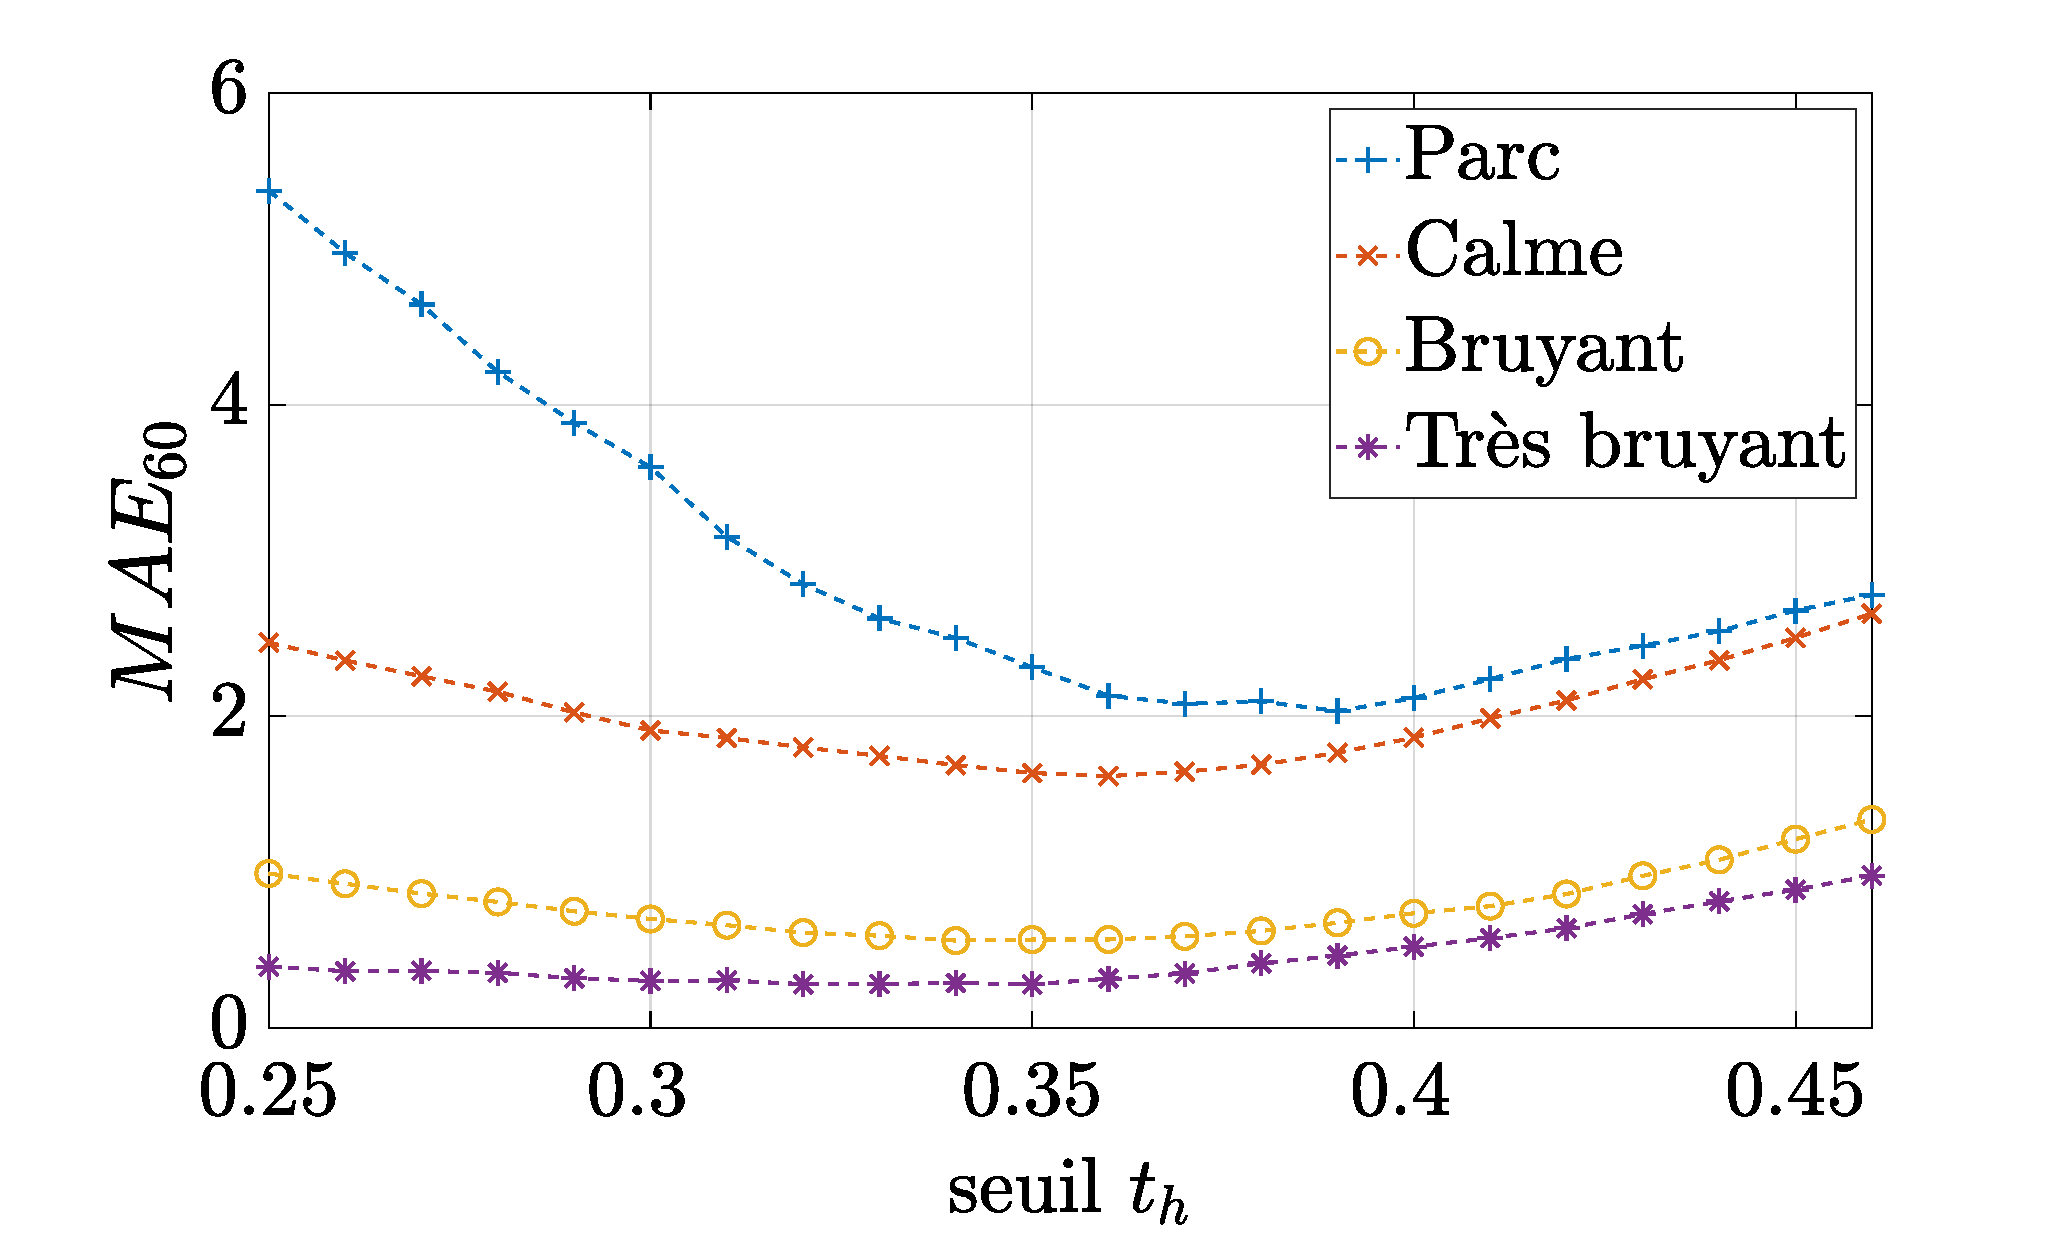
\includegraphics[width=.7\linewidth]{./figures/resultats/maeExpandseuil.pdf}
 \caption{Influence de la valeur seuil sur les erreurs $MAE_{60}$ selon l'ambiance sonore.}
 \label{fig:maeExpandSeuil}
 \end{figure}
  

Dans le cas de l'ambiance \textit{rue bruyante} et \textit{rue très bruyante}, les erreurs sont peu sensibles aux variations du seuil. Le dictionnaire est déjà composé d'un grand nombre d'éléments \textit{trafic}, la variation du seuil modifie ce nombre de 1 ou 2 éléments, ce qui est relativement faible par rapport à la taille du dictionnaire $\mathbf{W}_{trafic}$. 
De plus dans le cas de \textit{rue très bruyante}, si la diminution du seuil jusqu'à $t_h$ = 0,31, et donc l'augmentation du nombre d'éléments dans $\mathbf{W}_{trafic}$, permet, dans un premier temps, la diminution de l'erreur $MAE_{60}$, celle-ci devient par la suite quasi constante malgré la possibilité d'inclure dans $\mathbf{W}_{trafic}$ des éléments de la classe \textit{interférante}. 
L'impact de cette classe y est alors très faible puisqu'elle est très peu présente dans ces scènes sonores et que le nombre d'éléments \textit{trafic} étant beaucoup plus élevé, leur prise en compte dans $\mathbf{W}_{trafic}$ aura une influence très faible. 
Pour l'ambiance \textit{parc}, le choix de $t_{h,opt}$ est plus influent puisque l'évolution de l'erreur $MAE_{60}$ est plus sensible à la valeur du seuil. Cette sensibilité est d'autant plus forte que les valeurs seuils sont faibles en raison, ici, de la prédominance de la classe interférante. Son augmentation permet alors de limiter cette présence dans $\mathbf{W}_{trafic}$.

Ainsi, même si le choix d'utiliser des valeurs seuils optimales à l'ambiance sonore parait intéressant, la faible sensibilité de l'erreur $MAE_{60}$ pour les ambiances sonores \textit{rue calme}, \textit{rue bruyante} et \textit{rue très bruyante} ne permet pas d'avoir une diminution significative des erreurs. Cette amélioration est surtout présente pour l'ambiance \textit{parc} qui permet de limiter la présence d'éléments de la classe \textit{interférante} dans $\mathbf{W}_{trafic}$.
En annexe \ref{annexe:optThreshold} est présenté un travail menant à l'estimation d'un seuil optimal à l'aide d'indicateurs de niveau sonore. Le seuil optimale est ainsi non pas déterminé \textit{a priori} mais à partir de la valeur de cet indicateur corrélé à l'évolution des seuils optimaux $t_{h,opt}$ permettant ainsi de s'adapter à des environnements variables Si cette piste peut être utile dans le cas de réseaux où l'ambiance sonore n'est pas définie au préalable ou si l'environnement sonore évolue au cours du temps, elle ne permet pas d'améliorer suffisamment les estimations des niveaux sonores \textit{trafic} pour être considérée ici.

%\end{document}